\documentclass[12pt,a4paper]{report}

% Packages
\usepackage[utf8]{inputenc}
\usepackage[T5]{fontenc}
\usepackage[vietnamese,english]{babel}
\usepackage{graphicx}
\usepackage{geometry}
\usepackage{hyperref}
\usepackage{titlesec}
\usepackage{fancyhdr}
\usepackage{setspace}
\usepackage{mathptmx}
\usepackage{float}
\usepackage[utf8]{vietnam}
\usepackage{longtable}
\usepackage{array}
\usepackage{tikz}
\usepackage{pgfplots}
\pgfplotsset{compat=1.18}
\usepackage{rotating}

\addto\captionsenglish{%
  \renewcommand{\contentsname}{TABLE OF CONTENTS}
  \renewcommand{\listfigurename}{LIST OF FIGURES}
  \renewcommand{\listtablename}{LIST OF TABLES}
  \renewcommand{\bibname}{REFERENCES}
  \renewcommand{\figurename}{Figure}
  \renewcommand{\tablename}{Table}
}

% Page setup
\geometry{
    a4paper,
    left=30mm,
    right=20mm,
    top=25mm,
    bottom=25mm
}

\graphicspath{{images/}}
\onehalfspacing

% Header and Footer
\pagestyle{fancy}
\fancyhf{}
\rhead{\thepage}
\lhead{Smart Boarding House Management System}

\begin{document}

\newgeometry{left=25mm,right=25mm,top=25mm,bottom=25mm}
\begin{titlepage}
    \centering
    {\large \textbf{UNIVERSITY OF SCIENCE AND TECHNOLOGY OF HANOI} \par}
    \vspace{0.2cm}
    {\large \textbf{DEPARTMENT OF INFORMATION AND COMMUNICATION TECHNOLOGY} \par}
    \vspace{1.5cm}
    
\includegraphics[width=0.38\textwidth]{usth.png} \par
    \vspace{2cm}
    {\huge \textbf{SMART BOARDING HOUSE MANAGEMENT SYSTEM} \par}
    \vspace{1cm}
    {\Large \textbf{BACHELOR THESIS} \par}

    \vfill

    \begin{tabular}{@{}ll@{}}
        \textbf{Student:}             & Nguyễn Văn Linh \\[4pt]
        \textbf{Student ID:}          & 22BI13252 \\[4pt]
        \textbf{External Supervisor:} & Lê Văn Sơn \\[4pt]
        \textbf{Internal Supervisor:} & Trần Giang Sơn \\
    \end{tabular}

    \vfill

    {\large \textbf{Hanoi, June 2026} \par}
    \thispagestyle{empty}
\end{titlepage}
\restoregeometry

\pagenumbering{roman}

\thispagestyle{empty}

\begin{center}
    {\large To whom it may concern, \par}
\end{center}
\vspace{1cm}

\noindent I, \makebox[9.5cm]{\dotfill} (supervisor's name), certify that the thesis/ internship report of Mr/Ms. \makebox[8.5cm]{\dotfill} (student's name) is qualified to be presented in the Internship Jury 2025-2026.

\vspace{3cm}

\begin{flushright}
    Hanoi, 28/06/2026 \\
    \vspace{0.5cm}
    \textbf{Supervisor's signature}
\end{flushright}
\newpage

\chapter*{ACKNOWLEDGEMENTS}
\addcontentsline{toc}{chapter}{ACKNOWLEDGEMENTS}
\thispagestyle{empty}

I would like to express my gratitude to all those who gave me the possibility to complete this thesis, as well as the academic support that I received during the time of my studying at the University of Science and Technology of Hanoi (USTH).

Foremost, I would like to send my honest thanks to my supervisors, Assoc. Prof. Trần Giang Sơn (Internal Supervisor) and Dr. Lê Văn Sơn (External Supervisor). Their guidance, patience, and valuable feedback throughout the development of the \textbf{Smart Boarding House Management System} have been crucial to the completion of this bachelor thesis. Their insights into software architecture, database design, and systems engineering have greatly helped me improve both my academic knowledge and engineering skills.

I also want to thank the lecturers and staff of the Department of Information and Communication Technology (ICT) at USTH for providing me with a solid academic foundation and a supportive learning environment.

Finally, I would like to thank my family and friends for their constant encouragement, support, and understanding during my studies and the completion of this thesis project.

\vspace{1.5cm}
\begin{flushright}
Nguyễn Văn Linh
\end{flushright}
\newpage


\chapter*{ABSTRACT}
\addcontentsline{toc}{chapter}{ABSTRACT}
\selectlanguage{english}
This project is about building a website called Smart Boarding House Management System. It is a SaaS platform that helps landlords and tenants manage their rental activities together. The system solves common problems in boarding houses, such as different room information, writing contracts by hand, delay in calculating monthly bills, lack of communication between landlords and tenants, and difficulties in tracking room issues or tenant rules violations.

To build this website, NestJS is used for the backend and Next.js for the frontend. PostgreSQL with Prisma is used to store main information like rooms and contracts. MongoDB is also used to keep activity logs, and Socket.IO to send real-time notifications to users. The platform has private zones for landlords and tenants. It includes many features: managing rooms and tenants, keeping track of contracts, generating monthly invoices automatically, checking payment status, exporting PDF bills with VietQR payment codes, reporting room problems, tracking tenant violations, and using a smart AI assistant to chat with tenants or write notifications.

The result of the project is a helpful system that saves time for landlords. It also gives tenants an easy way to check their contracts, bills, payments, and to report problems. This project is a great way to learn clean coding architecture, modular frontend design, user access security, automated tasks, and how to connect AI helper to a real business system.

\newpage
\tableofcontents
\addcontentsline{toc}{chapter}{TABLE OF CONTENTS}
\newpage
\listoffigures
\addcontentsline{toc}{chapter}{LIST OF FIGURES}
\newpage
\listoftables
\addcontentsline{toc}{chapter}{LIST OF TABLES}
\newpage
\chapter*{LIST OF ABBREVIATIONS}
\addcontentsline{toc}{chapter}{LIST OF ABBREVIATIONS}

\begin{longtable}{@{}ll@{}}
\textbf{Abbreviation} & \textbf{Definition} \\
AI & Artificial Intelligence \\
API & Application Programming Interface \\
CRUD & Create, Read, Update, Delete \\
DTO & Data Transfer Object \\
HTTP & Hypertext Transfer Protocol \\
HTTPS & Hypertext Transfer Protocol Secure \\
JWT & JSON Web Token \\
ORM & Object-Relational Mapping \\
PDF & Portable Document Format \\
RBAC & Role-Based Access Control \\
REST & Representational State Transfer \\
SaaS & Software as a Service \\
SQL & Structured Query Language \\
UI & User Interface \\
URL & Uniform Resource Locator \\
UUID & Universally Unique Identifier \\
VND & Vietnamese Dong \\
WebSocket & Web-based full-duplex communication protocol \\
\end{longtable}


\pagenumbering{arabic}

\chapter{INTRODUCTION}

\section{Context and Motivation}
In Vietnam, many landlords of boarding houses and small rental buildings still manage their business using simple methods. They often use paper notebooks, \textbf{Excel} files, social chat applications, or check bank transfers manually. Although these methods are easy to use at first, they become very hard to manage when the landlord has more rooms and tenants. Landlords have to spend a lot of time doing things like updating room availability, collecting tenant information, writing contracts, calculating bills every month, tracking payments, answering questions, and fixing broken facilities or handling rules violations.

Using different simple tools at the same time causes many problems. For example, room information can be different between what landlords post online and what they write in their private logs. It is also difficult to find old contracts and payment history. Tenants do not have a place to check their rental information, payment status, and reported issues by themselves. Also, when landlords calculate and write bills by hand, they can easily forget deadlines, make mistakes in calculations, or send payment notifications late.

Therefore, this project aims to build a website called \textbf{Smart Boarding House Management System} to put all these tasks together in one \textbf{SaaS} platform. This system has three main parts: a \textbf{public page} to show available rooms, a \textbf{landlord dashboard}, and a \textbf{tenant portal}. The system also has automatic and smart features like creating bills on schedule, creating \textbf{PDF} invoices with \textbf{VietQR} payment codes, sending notifications, and using \textbf{AI} to chat with users or generate announcements.

\section{Project Overview}
The system has two main user groups: \textbf{landlords} and \textbf{tenants}. The first group is \textbf{landlords}, who can manage rooms, tenants, contracts, invoices, reported incidents, consultation requests, and tenant violations. The second group is \textbf{tenants}, who can view their current contract, track their invoices, report room incidents, receive notifications, and chat with an \textbf{AI} assistant that understands their rental details.

For the \textbf{backend}, \textbf{NestJS} is used to build a modular system. The system is organized into different modules like login, rooms, tenants, contracts, invoices, rent requests, incidents, violations, PDF generation, upload, notification, and AI assistant. The \textbf{frontend} is built using \textbf{Next.js}. It is divided into public pages, login pages, a landlord admin dashboard, and a tenant portal.

\section{Report Structure}
This report is divided into six chapters:

\begin{itemize}
    \item \textbf{Chapter 1 (Introduction):} Introduces the project, its background, reasons for development, and system overview.
    \item \textbf{Chapter 2 (Objectives):} Describes the objectives, functional goals, scope of work, and expected results.
    \item \textbf{Chapter 3 (Requirements Analysis):} Shows the requirements analysis, including user roles, system requirements, use cases, and database details.
    \item \textbf{Chapter 4 (Methodology):} Explains the methodology, such as the chosen technologies, application architecture, database model, and step-by-step implementation.
    \item \textbf{Chapter 5 (Results and Discussion):} Discusses the results, focusing on the implemented features, testing, and limitations.
    \item \textbf{Chapter 6 (Conclusion and Future Work):} Concludes the report and suggests some future improvements.
\end{itemize}


\chapter{OBJECTIVES}

\section{Desired Features}
The main goal of this project is to build a website for managing rental houses. The website helps manage everything from showing vacant rooms to the public, adding tenants, writing contracts, creating monthly bills, tracking payments, reporting issues, and helping landlords and tenants communicate easily.

\subsection{Public Rental Interface}
The public page allows people who want to rent a room to look at available rooms and send requests for consultation. It only shows vacant rooms and gives details like the price, room status, and description. In addition, a smart \textbf{AI} helper can answer common questions from users by using the room data in the database.

\subsection{Landlord Administration Dashboard}
The \textbf{landlord dashboard} is the main control center of the website. It gives \textbf{landlords} tools to manage rooms, add new tenants, write rental contracts, create monthly invoices, update payment status, manage room issues, track violations, and read room requests. The dashboard also keeps data private. This means each landlord can only see their own rooms, tenants, contracts, and invoices, and cannot see information from other landlords.

\subsection{Tenant Portal}
The \textbf{tenant portal} is a personal page for renters. Tenants can log in to check their contracts, see past bills, report issues in their rooms, read violation notices, mark invoices as paid, and get support from an \textbf{AI} assistant. This makes the rental process transparent and helps landlords and tenants save time because they do not have to ask the same questions repeatedly.

\section{Project Scope}
This project is designed for small and medium boarding houses, not for large real-estate companies. The main features in this project include user login with different roles for \textbf{landlords} and \textbf{tenants}, and keeping data private for each landlord. It also allows landlords to manage rooms and upload images, manage tenant accounts, and track contract status. In addition, the system can create monthly invoices automatically, export \textbf{PDF} bills, and show \textbf{VietQR} codes based on the landlord's bank account. Landlords can also track room incidents or tenant violations. Finally, the system sends real-time notifications to users and uses an \textbf{AI} assistant to support tenants and help landlords write notices.

\section{Engineering Goals}
Apart from building the application features, this project aims to achieve several engineering goals. First, the backend uses \textbf{Clean Architecture} rules and is built with \textbf{NestJS}. Second, the frontend is built with \textbf{Next.js} and has private pages. Third, \textbf{PostgreSQL} database with \textbf{Prisma} is used to keep all data consistent. The system also uses \textbf{JWT} and security guards to protect the API routes. Moreover, scheduled cron jobs are used to create monthly invoices and check expired contracts automatically. Finally, the system connects with third-party services like \textbf{Cloudinary} for image upload, \textbf{Google Generative AI} for the assistant, and \textbf{Socket.IO} for real-time messages.

\section{Expected Outcomes}
The expected result is a working prototype of a rental \textbf{SaaS} platform. This prototype can be a good foundation to build a complete boarding house management system in the future. For \textbf{landlords}, the system will reduce manual paperwork and make it easier to see how their business is running. For \textbf{tenants}, the system will help them check their bills, payment status, and get support easily and quickly.

\chapter{REQUIREMENTS ANALYSIS}

\section{Overall System Requirements}
The system is designed around three access contexts: \textbf{public visitors}, \textbf{landlords}, and \textbf{tenants}. Each context has different permissions and workflows.

\subsection{Public Visitor Requirements}
\textbf{Public visitors} do not need to log in. They must be able to browse vacant rooms, view room information, submit consultation requests, and ask basic questions through the public \textbf{AI} assistant.

\subsection{Landlord Requirements}
\textbf{Landlords} must authenticate before accessing the \textbf{administration dashboard}. For landlords, the system requires several core features. First, landlords need room management to create, update, delete, list, and upload images of rooms. Rooms can have status like \textbf{vacant}, \textbf{occupied}, or \textbf{maintenance}. Second, landlords need tenant management to view tenants, approve or reject tenant registration requests, and connect tenants with rooms. Third, contract management is necessary to create rental contracts, record rental price and deposit, and update contract status. Fourth, invoice management allows landlords to create bills, review payment history, check payment status, and export invoices to \textbf{PDF} files. Fifth, operational support helps landlords review room incidents, track tenant violations, and receive real-time notifications. Finally, landlords can use \textbf{AI} assistance to generate announcements and notices for tenants quickly.

\subsection{Tenant Requirements}
\textbf{Tenants} must authenticate before accessing private rental information. For tenants, the system requires access to private rental data after they log in. Tenants must be able to view their active and past contracts, check invoices, and see if they have paid. They also need to mark invoices as paid so that the landlord can check and confirm their payment. If there is a problem in the room, tenants must be able to report incidents. Additionally, they can see violation notices and ask questions to the \textbf{AI} assistant about their contract or bills.

\section{Use Cases}

\subsection{Landlord Use Case}
The landlord actor manages the boarding house operation through the administration dashboard. The main workflow groups are room management, tenant management, contract and invoice processing, rent request handling, and operational support.

\begin{figure}[H]
    \centering
    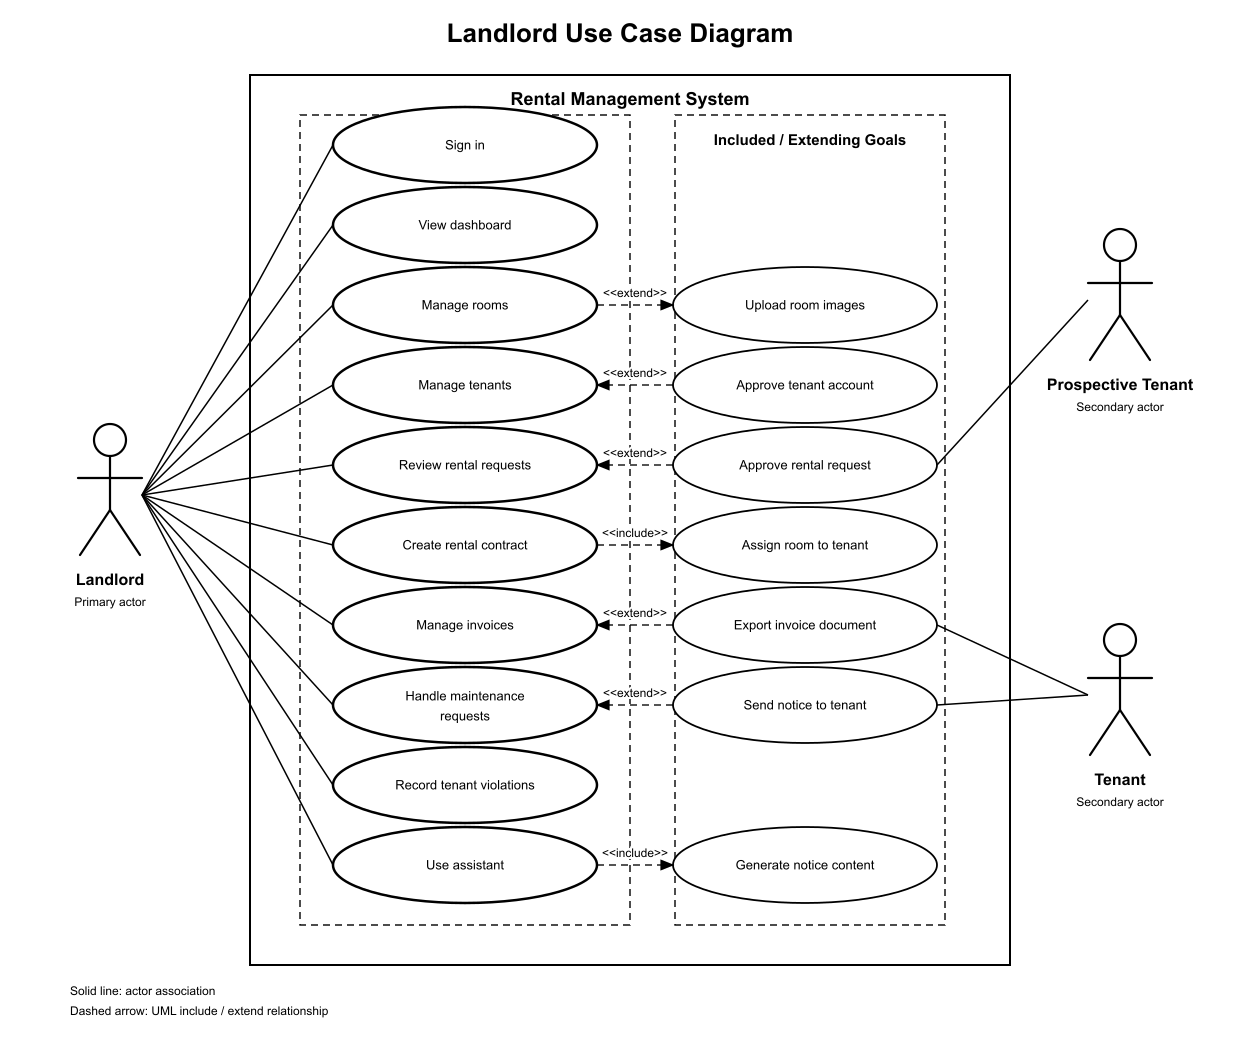
\includegraphics[width=0.95\textwidth]{landlord_usecase.png}
    \caption{Use Case Diagram - Landlord Administration Dashboard}
    \label{fig:landlord_usecase}
\end{figure}

\begin{table}[H]
    \centering
    \renewcommand{\arraystretch}{1.2}
    \begin{tabular}{|l|l|p{8cm}|}
        \hline
        \textbf{ID} & \textbf{Use Case Name} & \textbf{Description} \\
        \hline
        UC-LAN-01 & Manage rooms & Create, edit, delete, and update room availability. \\
        \hline
        UC-LAN-02 & Manage tenants & Review tenant accounts and tenant information. \\
        \hline
        UC-LAN-03 & Manage contracts & Create and update rental contracts. \\
        \hline
        UC-LAN-04 & Manage invoices & Create invoices, update payment status, and export invoice PDFs. \\
        \hline
        UC-LAN-05 & Handle incidents & Review and update tenant-reported maintenance requests. \\
        \hline
        UC-LAN-06 & Track violations & Record and resolve tenant violations. \\
        \hline
        UC-LAN-07 & Use AI assistance & Generate formal announcements and notices for tenants using the AI service. \\
        \hline
    \end{tabular}
    \caption{Summary of Landlord Use Cases}
    \label{tab:uc_summary_landlord}
\end{table}

\subsection{Tenant Use Case}
The tenant actor uses the portal to monitor their rental relationship with the landlord, especially contract and payment information.

\begin{figure}[H]
    \centering
    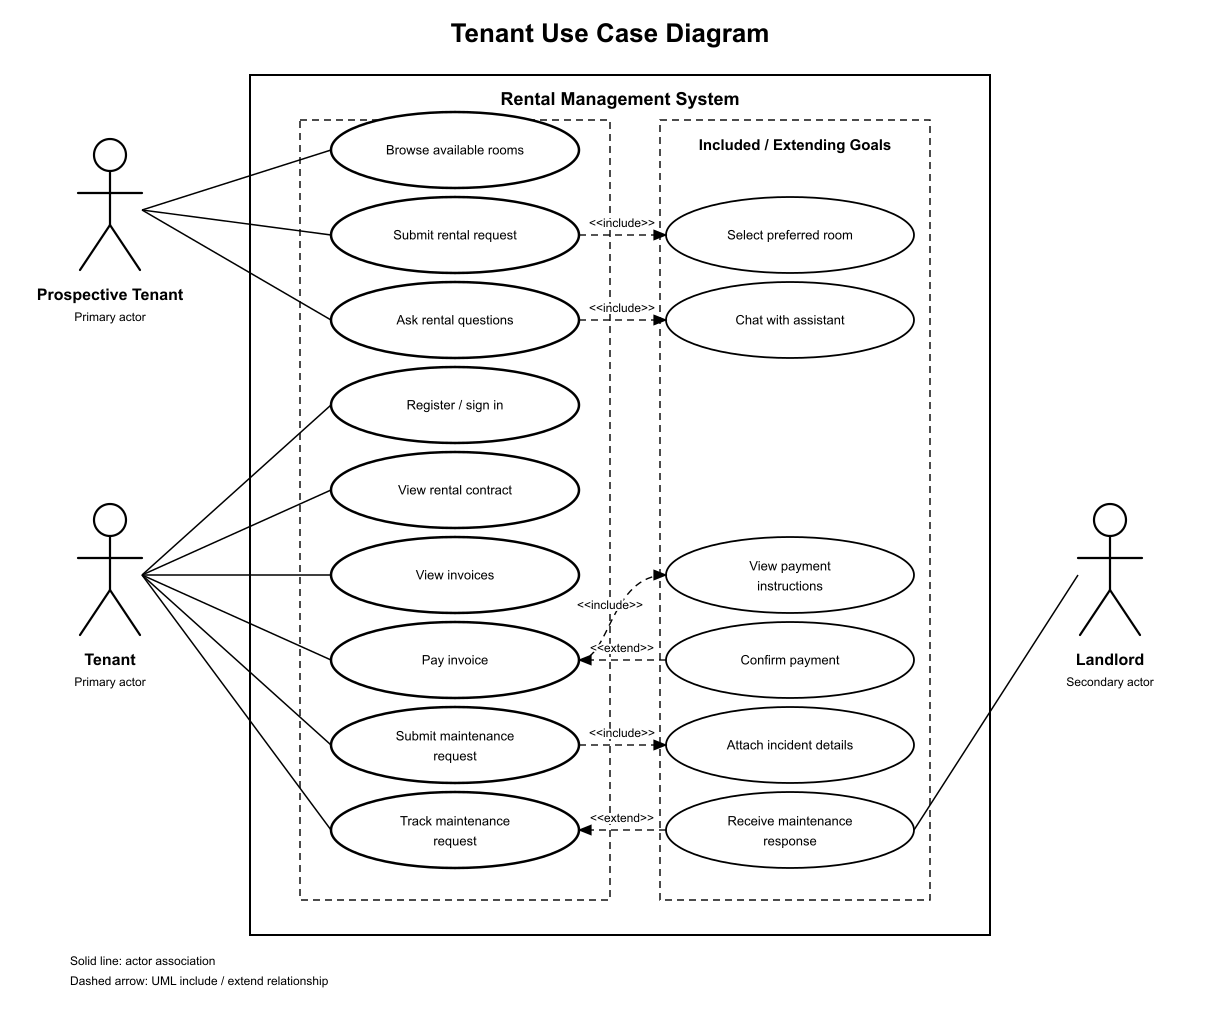
\includegraphics[width=0.95\textwidth]{tenant_usecase.png}
    \caption{Use Case Diagram - Tenant Portal}
    \label{fig:tenant_usecase}
\end{figure}

\begin{table}[H]
    \centering
    \renewcommand{\arraystretch}{1.2}
    \begin{tabular}{|l|l|p{8cm}|}
        \hline
        \textbf{ID} & \textbf{Use Case Name} & \textbf{Description} \\
        \hline
        UC-TEN-01 & Log in & Authenticate and access the tenant portal. \\
        \hline
        UC-TEN-02 & View contract & Review active rental contract information. \\
        \hline
        UC-TEN-03 & View invoices & Track invoices, due dates, and payment status. \\
        \hline
        UC-TEN-04 & Report incident & Submit a repair or support request for the rented room. \\
        \hline
        UC-TEN-05 & Use AI assistant & Ask contextual questions based on contract and invoice data. \\
        \hline
    \end{tabular}
    \caption{Summary of Tenant Use Cases}
    \label{tab:uc_summary_tenant}
\end{table}

\section{Use Case Specifications}
This section provides a detailed description of the execution operations for specific Use Cases, outlining the interaction steps between the user and the system components.

\subsection{Tenant Portal Use Cases}

\subsubsection{Tenant Log in}
\textbf{Goal:} To allow tenants and landlords to log in to their account.

\noindent \textbf{Primary Actor:} Tenant or Landlord

\noindent \textbf{Pre-conditions:} The user has registered an account with a valid email and password, and has a device connected to the internet.

\noindent \textbf{Main Success Scenario:}
\begin{enumerate}
    \item The user enters their email and password into the input fields.
    \item The user clicks the "Log In" button.
    \item The frontend validates the input format.
    \item The system sends a request to the backend auth service.
    \item The backend validates the credentials against the database.
    \item The system generates a JWT token and returns it to the user.
    \item The user is redirected to their dashboard page.
\end{enumerate}

\noindent \textbf{Alternative Flows:}
If the email or password is wrong, the system shows an incorrect password error and prompts the user to enter again. If there is a network error, the app displays a connection failure message.

\begin{figure}[H]
    \centering
    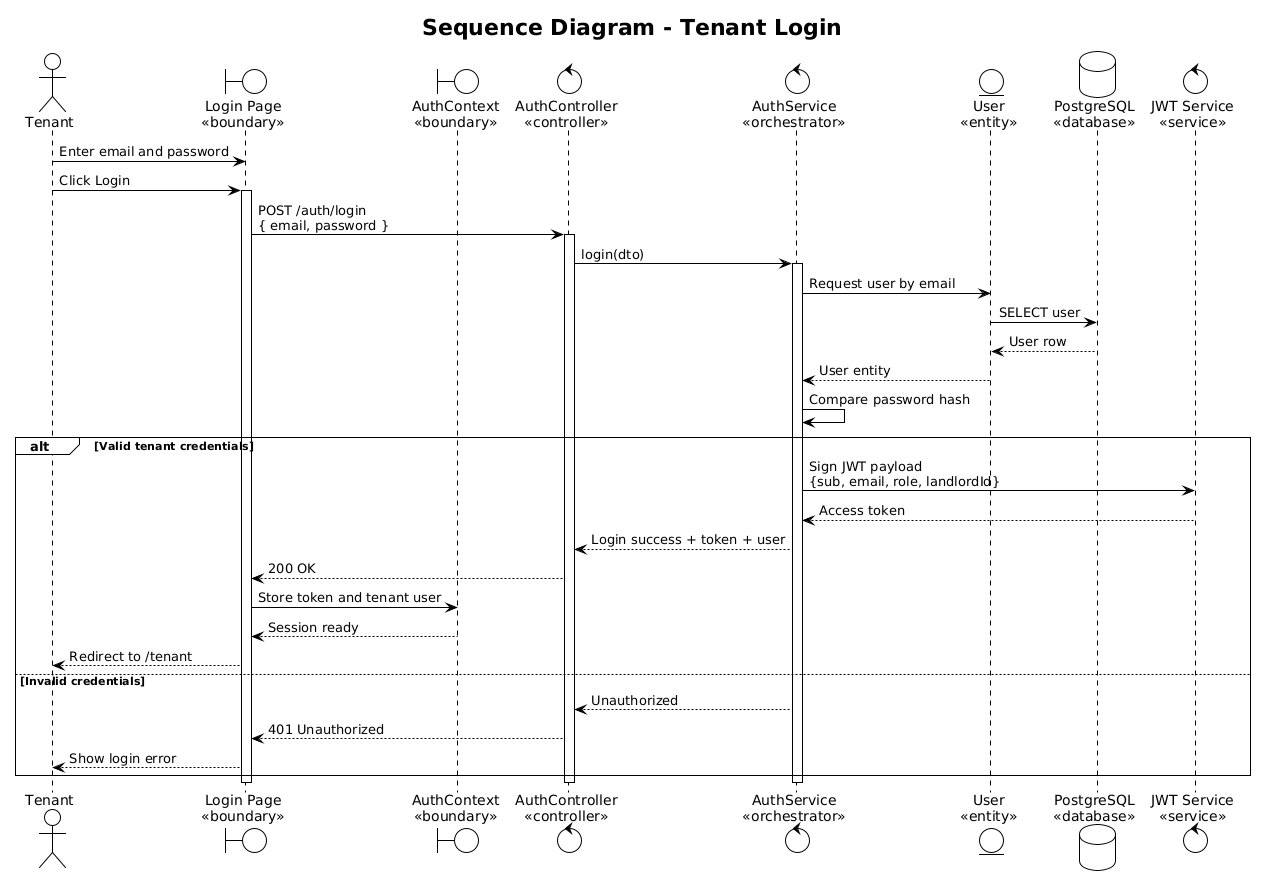
\includegraphics[width=0.9\textwidth]{seq_tenant_login.png}
    \caption{Sequence Diagram - Tenant Log in}
    \label{fig:seq_tenant_login}
\end{figure}

\subsubsection{View Contract}
\textbf{Goal:} To allow the tenant to review their current rental contract details.

\noindent \textbf{Primary Actor:} Tenant

\noindent \textbf{Pre-conditions:} The tenant is logged in.

\noindent \textbf{Main Success Scenario:}
\begin{enumerate}
    \item The tenant clicks the contract tab in the portal.
    \item The frontend sends a request with the JWT token to the backend.
    \item The backend fetches the contract details from the database.
    \item The system displays the start date, end date, rental price, and deposit.
\end{enumerate}

\noindent \textbf{Alternative Flows:}
If the contract is not found or has expired, the system shows a message that there is no active contract.

\begin{figure}[H]
    \centering
    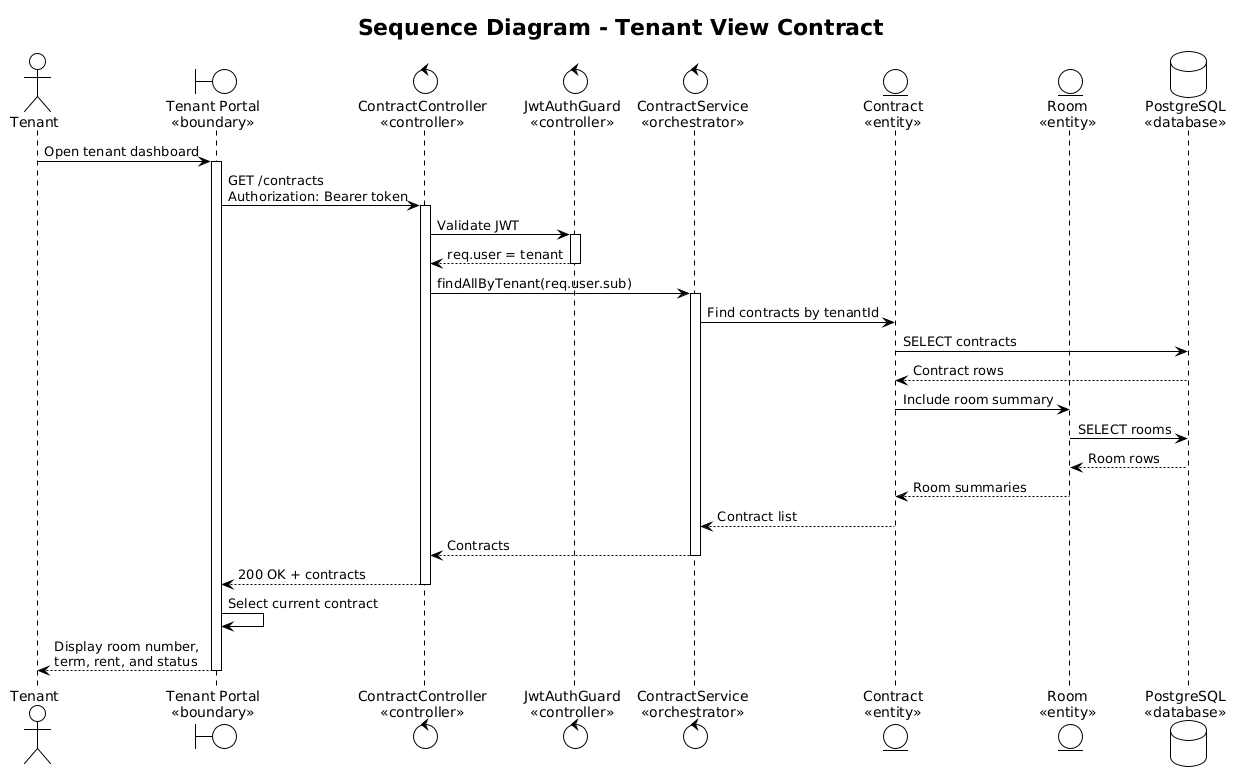
\includegraphics[width=0.9\textwidth]{seq_tenant_view_contract.png}
    \caption{Sequence Diagram - View Contract}
    \label{fig:seq_tenant_view_contract}
\end{figure}

\subsubsection{View Invoices}
\textbf{Goal:} To check invoice history and payment status.

\noindent \textbf{Primary Actor:} Tenant

\noindent \textbf{Pre-conditions:} The tenant is logged in.

\noindent \textbf{Main Success Scenario:}
\begin{enumerate}
    \item The tenant clicks on the billing section.
    \item The frontend sends a request with the JWT token to the backend.
    \item The backend queries the database for all invoices related to the tenant's contract.
    \item The system displays the list of invoices with their status like unpaid, paid, or overdue.
\end{enumerate}

\noindent \textbf{Alternative Flows:}
If the tenant has no invoices yet, the page shows an empty list.

\begin{figure}[H]
    \centering
    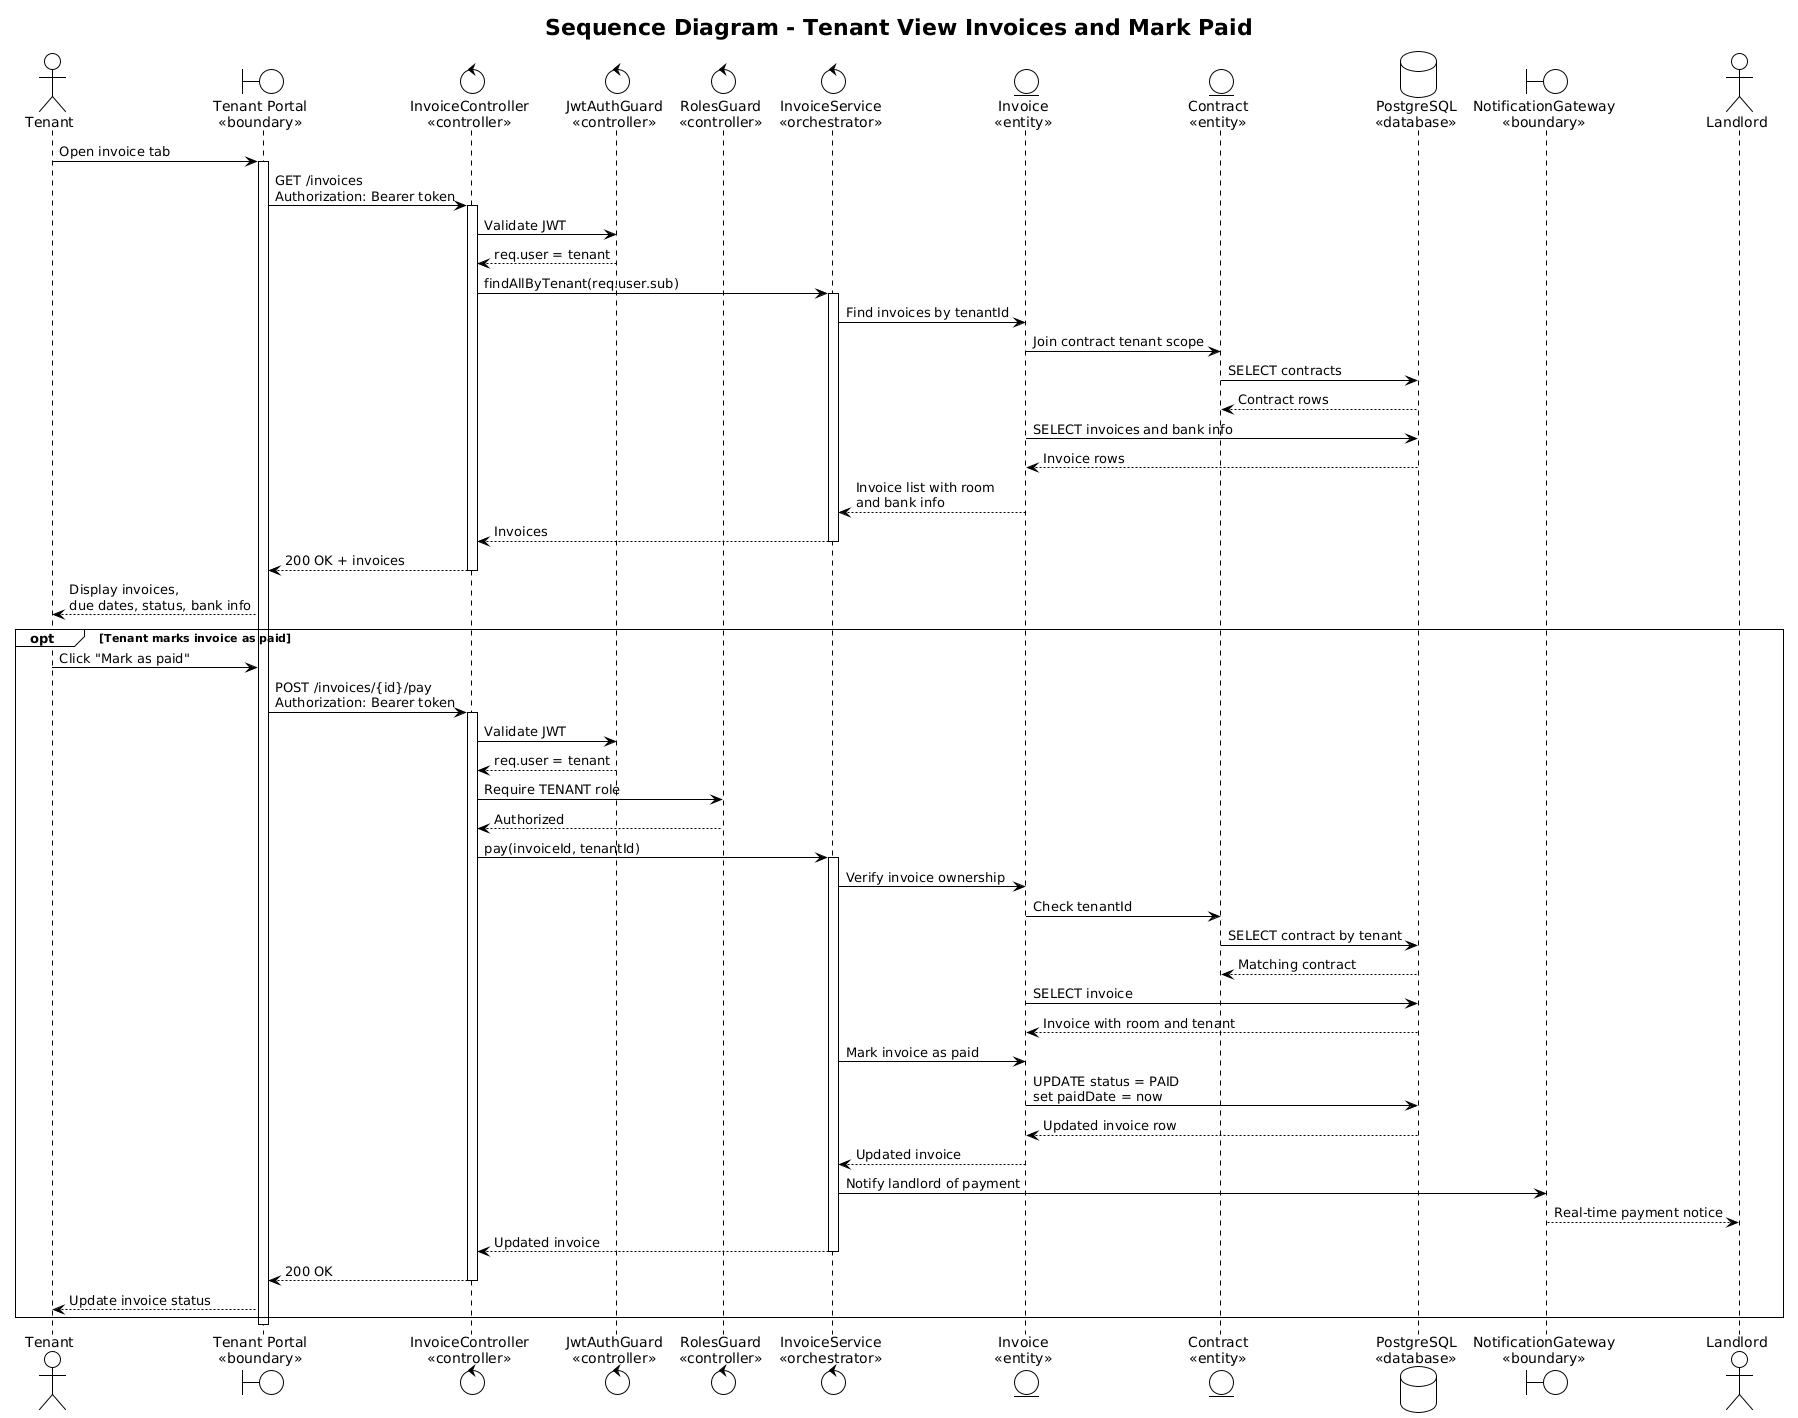
\includegraphics[width=0.9\textwidth]{seq_tenant_view_invoices.png}
    \caption{Sequence Diagram - View Invoices}
    \label{fig:seq_tenant_view_invoices}
\end{figure}

\subsubsection{Report Incident}
\textbf{Goal:} To submit a room maintenance issue to the landlord.

\noindent \textbf{Primary Actor:} Tenant

\noindent \textbf{Pre-conditions:} The tenant is logged in.

\noindent \textbf{Main Success Scenario:}
\begin{enumerate}
    \item The tenant opens the incident report form.
    \item The tenant enters the title, description, and selects the priority level.
    \item The tenant submits the form.
    \item The system saves the incident in the database and updates the status to pending.
    \item The system notifies the landlord in real time.
\end{enumerate}

\noindent \textbf{Alternative Flows:}
If the description is empty, the system prevents the submission and shows a validation error.

\begin{figure}[H]
    \centering
    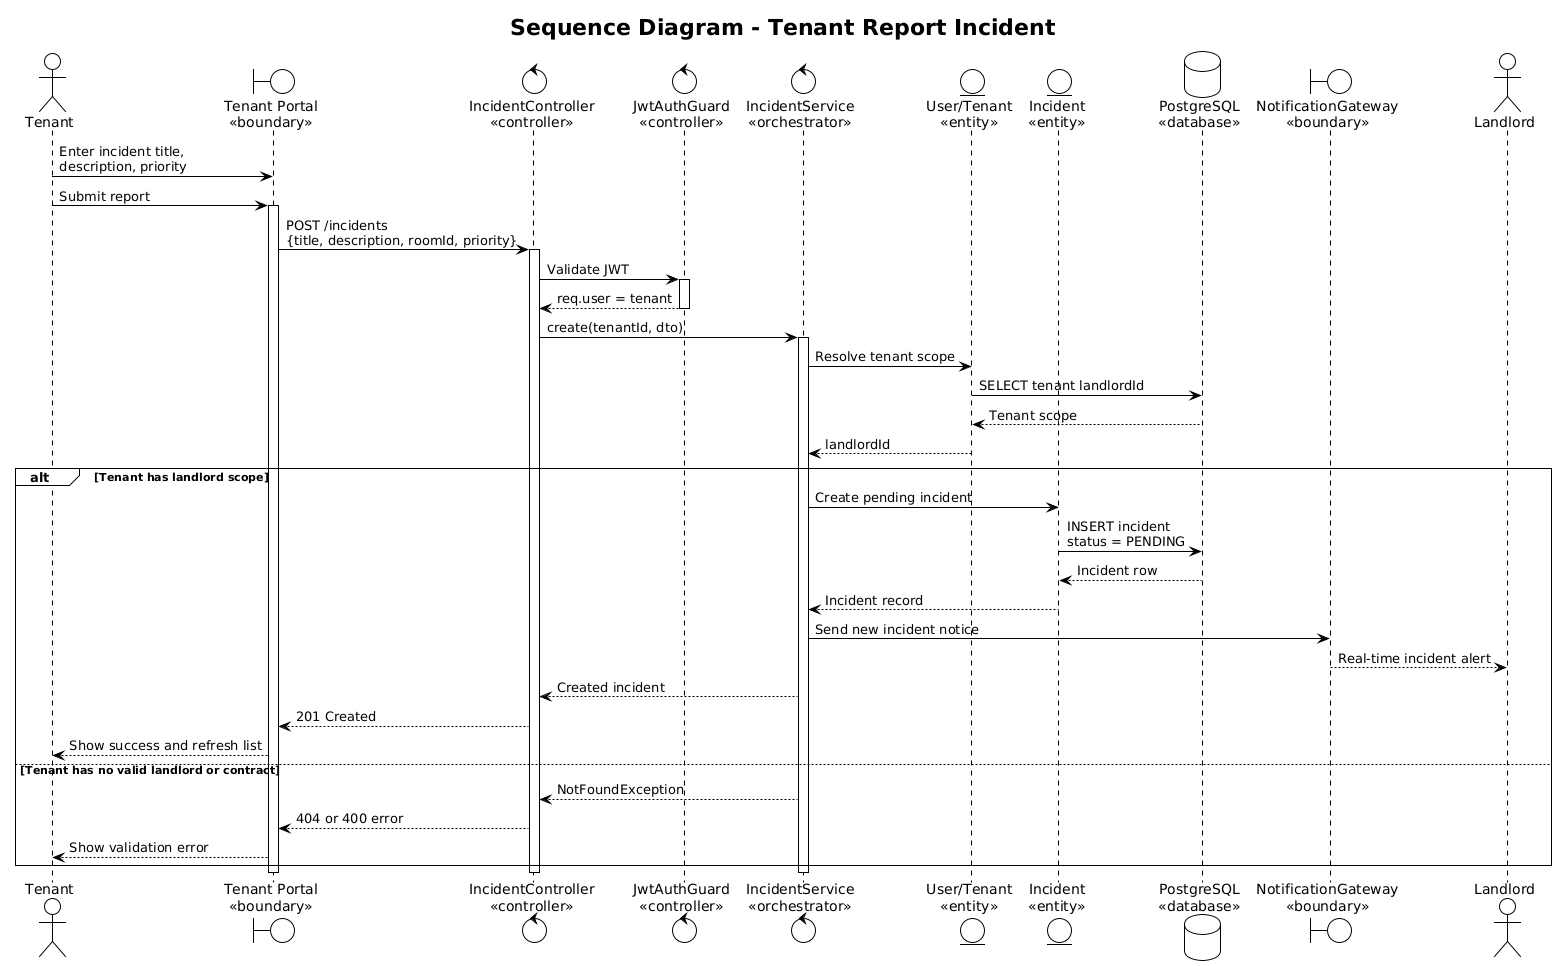
\includegraphics[width=0.9\textwidth]{seq_tenant_report_incident.png}
    \caption{Sequence Diagram - Report Incident}
    \label{fig:seq_tenant_report_incident}
\end{figure}

\subsubsection{Use AI Assistant}
\textbf{Goal:} To chat with an AI assistant that knows the tenant's rental details.

\noindent \textbf{Primary Actor:} Tenant

\noindent \textbf{Pre-conditions:} The tenant is logged in.

\noindent \textbf{Main Success Scenario:}
\begin{enumerate}
    \item The tenant opens the AI assistant chat box.
    \item The tenant writes a question about their rental terms.
    \item The backend fetches the tenant's contract and invoice data.
    \item The backend sends the question and the fetched data to the Google Gemini model.
    \item The model generates a response, and the system displays it to the tenant.
\end{enumerate}

\noindent \textbf{Alternative Flows:}
If the AI service is busy or not working, the system returns a message asking the user to try again later.

\begin{figure}[H]
    \centering
    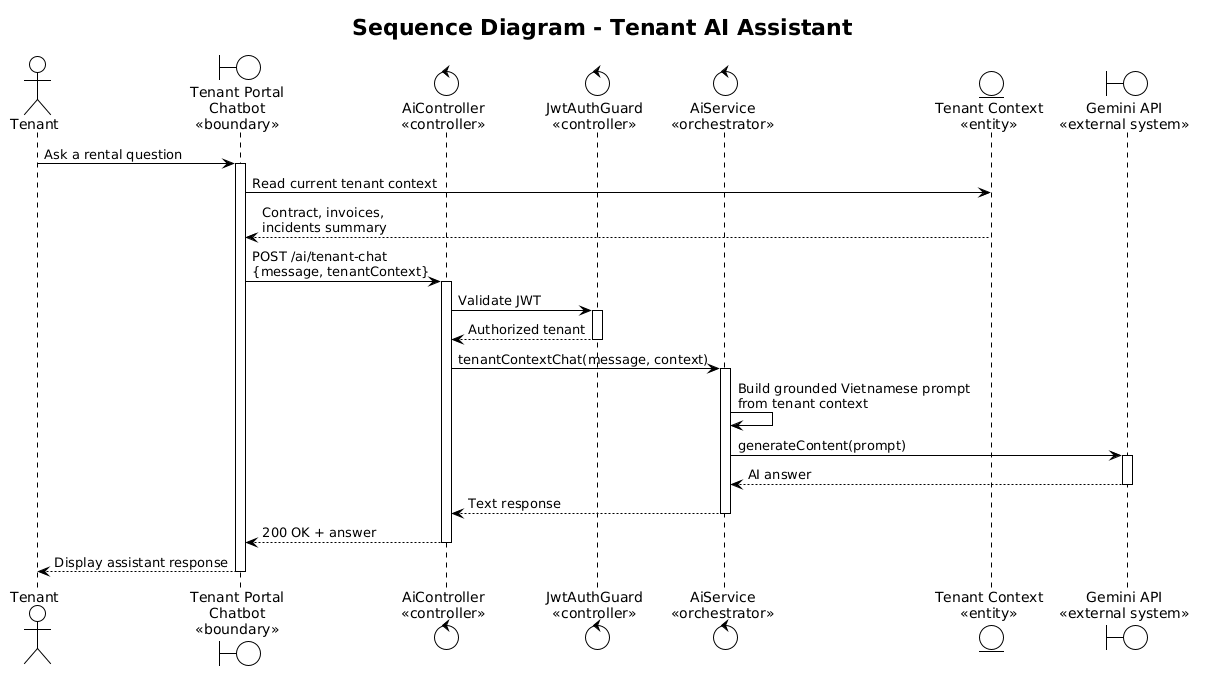
\includegraphics[width=0.9\textwidth]{seq_tenant_ai_assistant.png}
    \caption{Sequence Diagram - Use AI Assistant}
    \label{fig:seq_tenant_ai_assistant}
\end{figure}


\subsection{Landlord Dashboard Use Cases}

\subsubsection{Manage Rooms}
\textbf{Goal:} To create, update, or delete room listings.

\noindent \textbf{Primary Actor:} Landlord

\noindent \textbf{Pre-conditions:} The landlord is logged in.

\noindent \textbf{Main Success Scenario:}
\begin{enumerate}
    \item The landlord clicks on the room management menu.
    \item The landlord enters room details like room number, floor, price, description, and uploads images.
    \item The landlord clicks "Save".
    \item The backend saves the room information and uploads images to Cloudinary.
    \item The updated room list is displayed.
\end{enumerate}

\noindent \textbf{Alternative Flows:}
If the room number already exists, the system returns a validation error.

\begin{figure}[H]
    \centering
    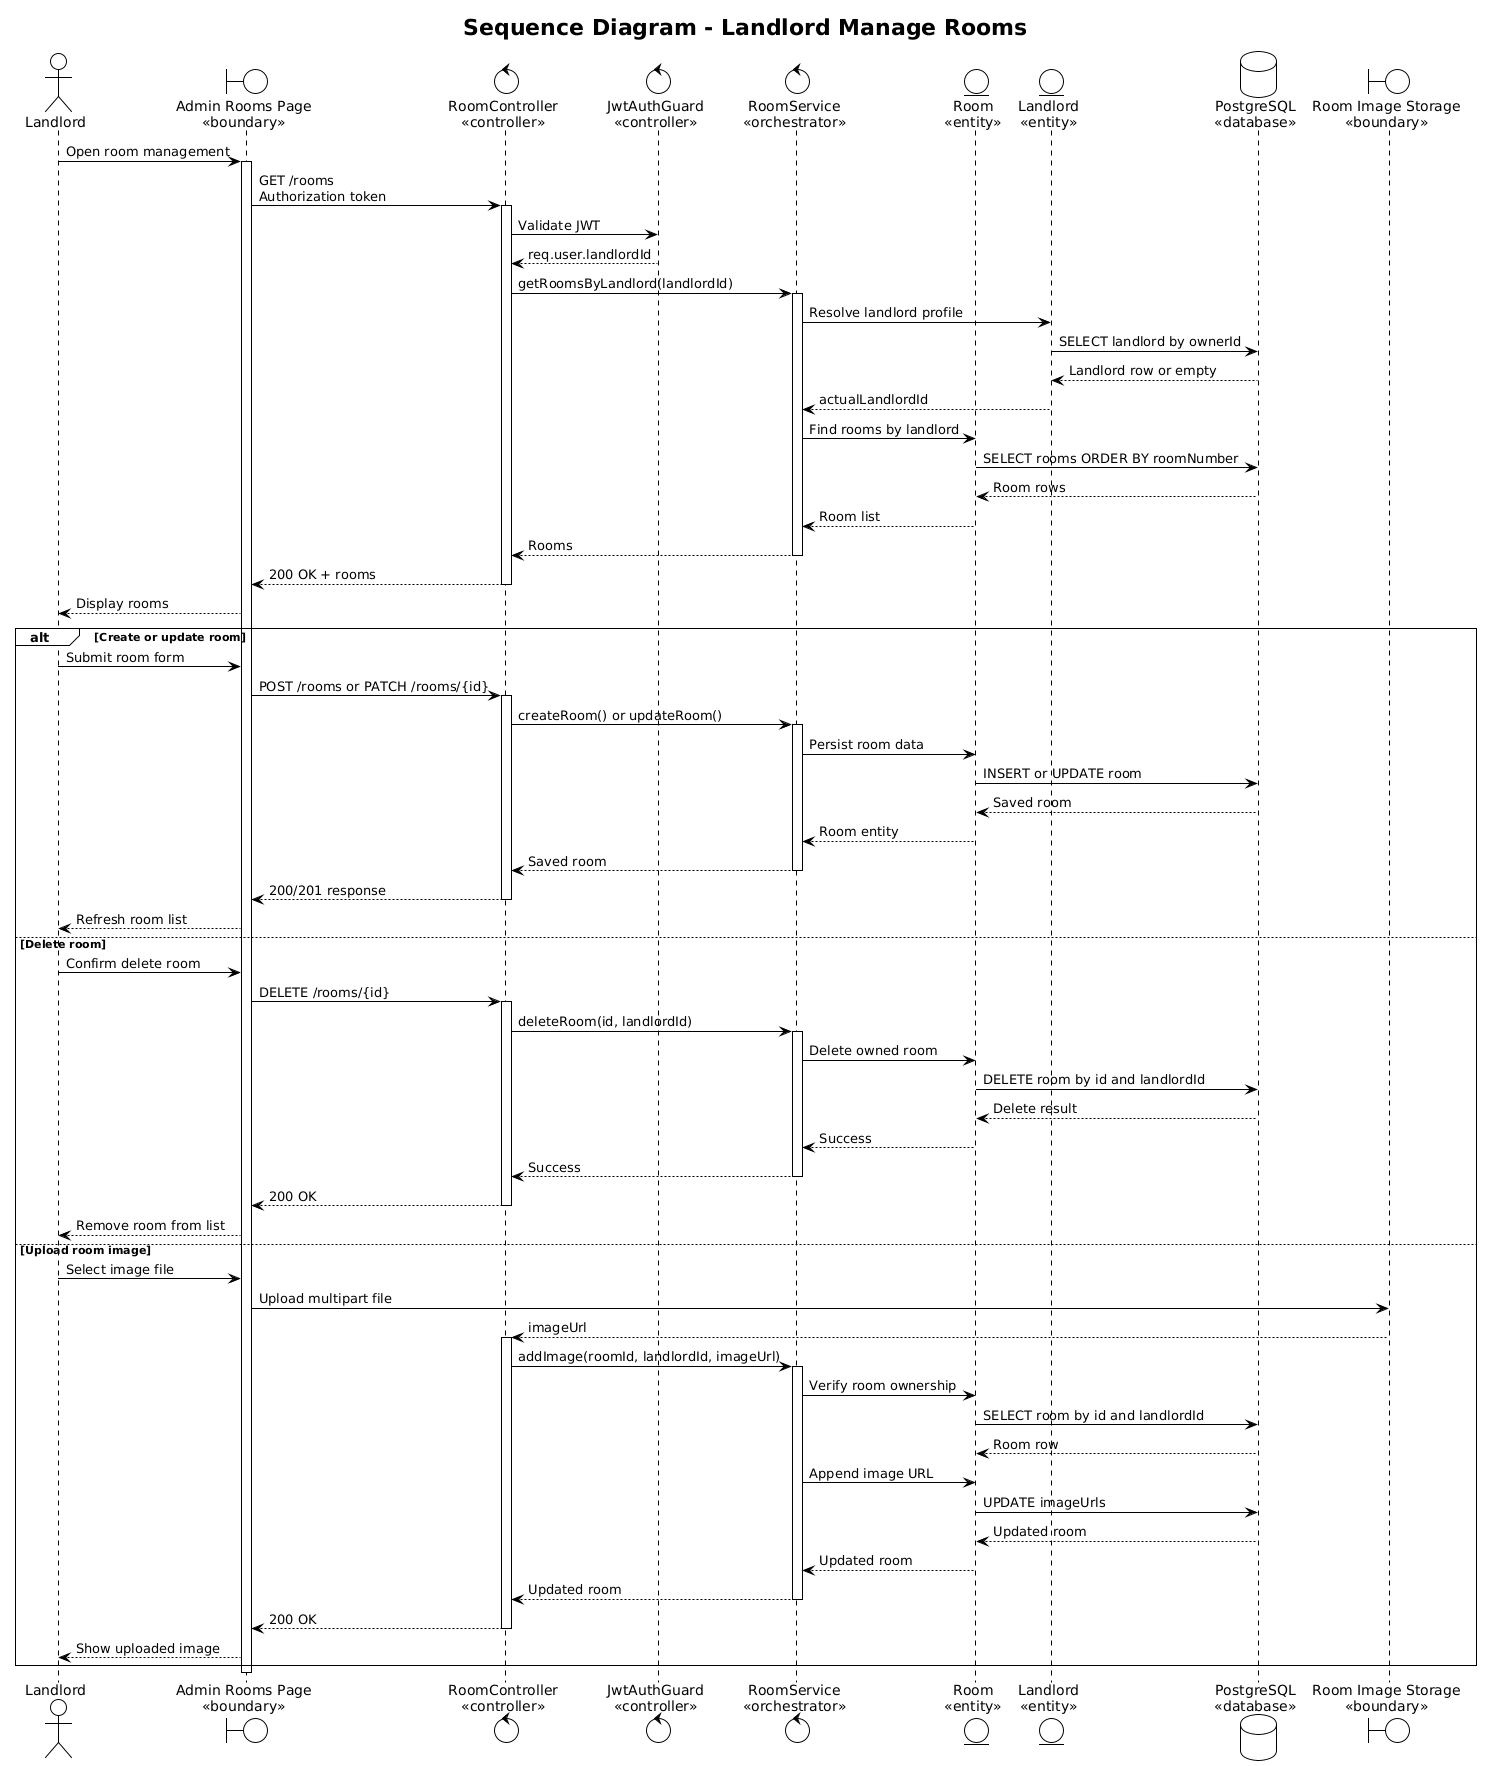
\includegraphics[width=0.9\textwidth]{seq_landlord_manage_rooms.png}
    \caption{Sequence Diagram - Manage Rooms}
    \label{fig:seq_landlord_manage_rooms}
\end{figure}

\subsubsection{Manage Tenants}
\textbf{Goal:} To approve and manage tenant accounts.

\noindent \textbf{Primary Actor:} Landlord

\noindent \textbf{Pre-conditions:} The landlord is logged in.

\noindent \textbf{Main Success Scenario:}
\begin{enumerate}
    \item The landlord opens the tenant management page.
    \item The landlord reviews the list of registered tenants and registration requests.
    \item The landlord approves a tenant.
    \item The system updates the tenant status in the database.
\end{enumerate}

\noindent \textbf{Alternative Flows:}
If the tenant's information is incomplete, the landlord can reject or suspend the account.

\begin{figure}[H]
    \centering
    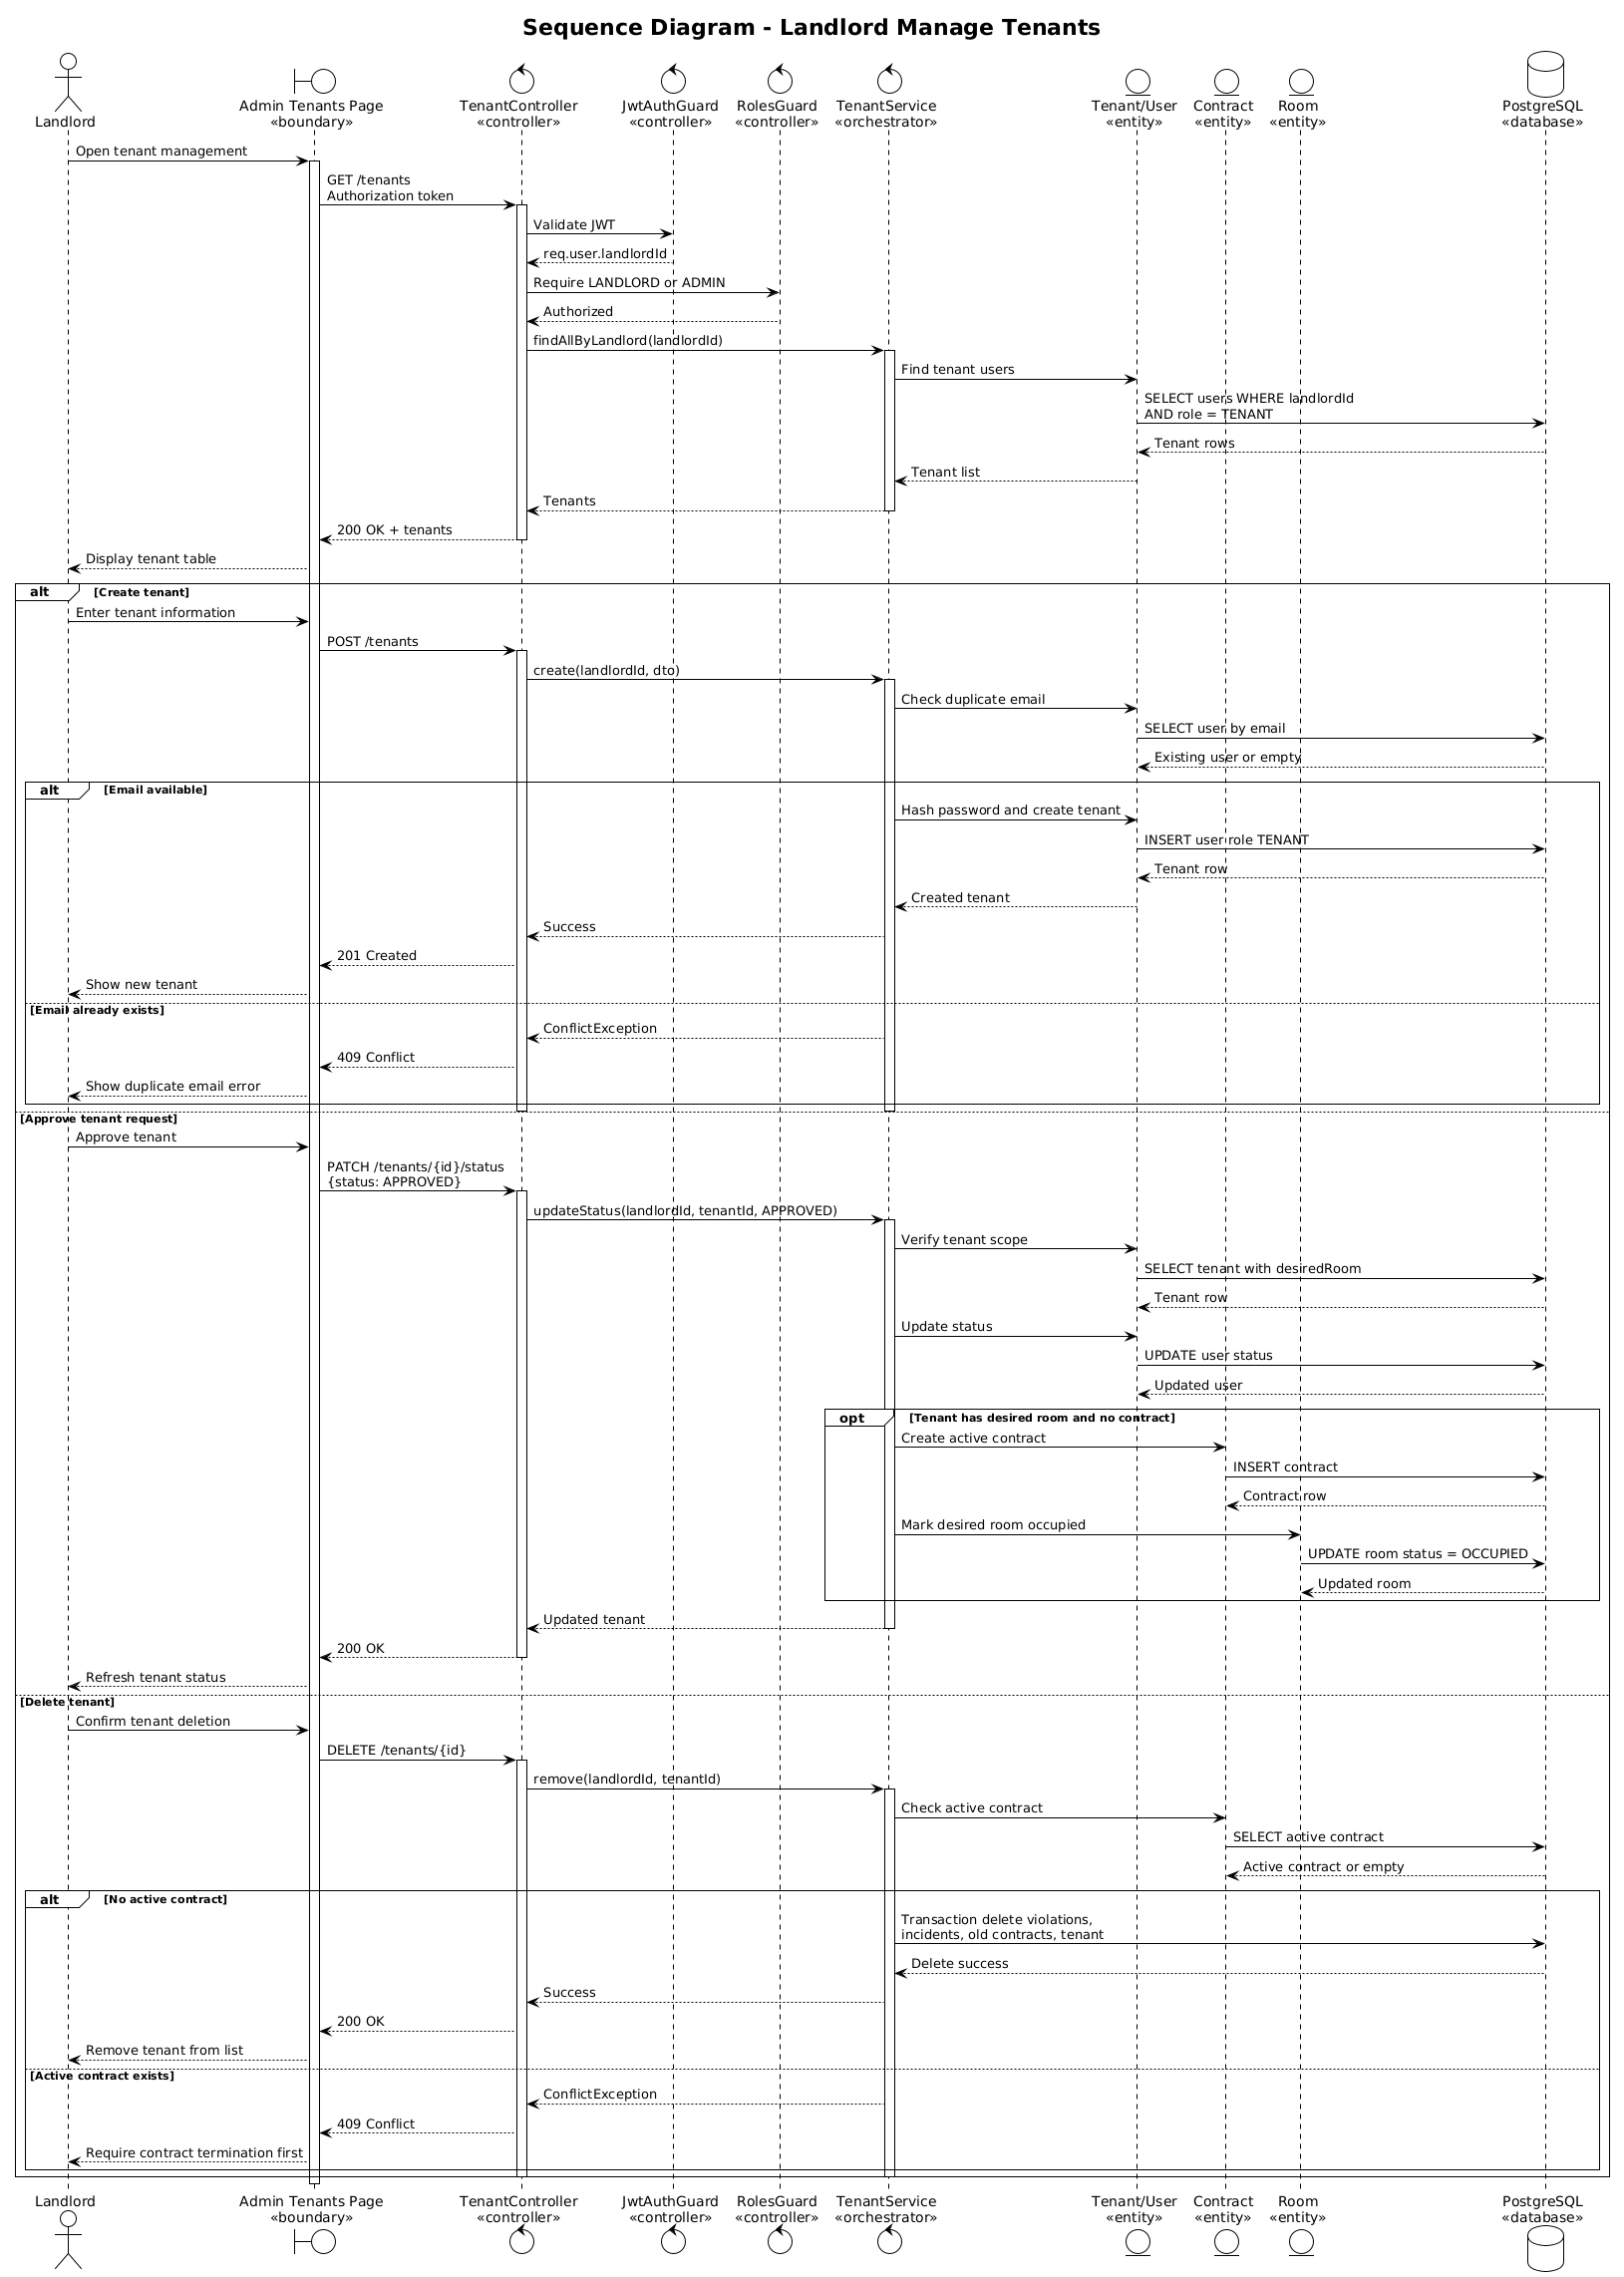
\includegraphics[width=0.9\textwidth]{seq_landlord_manage_tenants.png}
    \caption{Sequence Diagram - Manage Tenants}
    \label{fig:seq_landlord_manage_tenants}
\end{figure}

\subsubsection{Manage Contracts}
\textbf{Goal:} To create a rental contract between a tenant and a room.

\noindent \textbf{Primary Actor:} Landlord

\noindent \textbf{Pre-conditions:} The landlord is logged in. The room must be vacant, and the tenant must be approved.

\noindent \textbf{Main Success Scenario:}
\begin{enumerate}
    \item The landlord enters contract details like tenant, room, dates, deposit, and rental price.
    \item The landlord clicks "Save".
    \item The backend validates tenant ownership and room status.
    \item The system creates the contract inside a transaction.
    \item The room status is updated to occupied.
    \item The contract is shown in the dashboard.
\end{enumerate}

\noindent \textbf{Alternative Flows:}
If the room is occupied, the system rejects the request. If the tenant does not belong to this landlord, the system returns a validation error.

\begin{figure}[H]
    \centering
    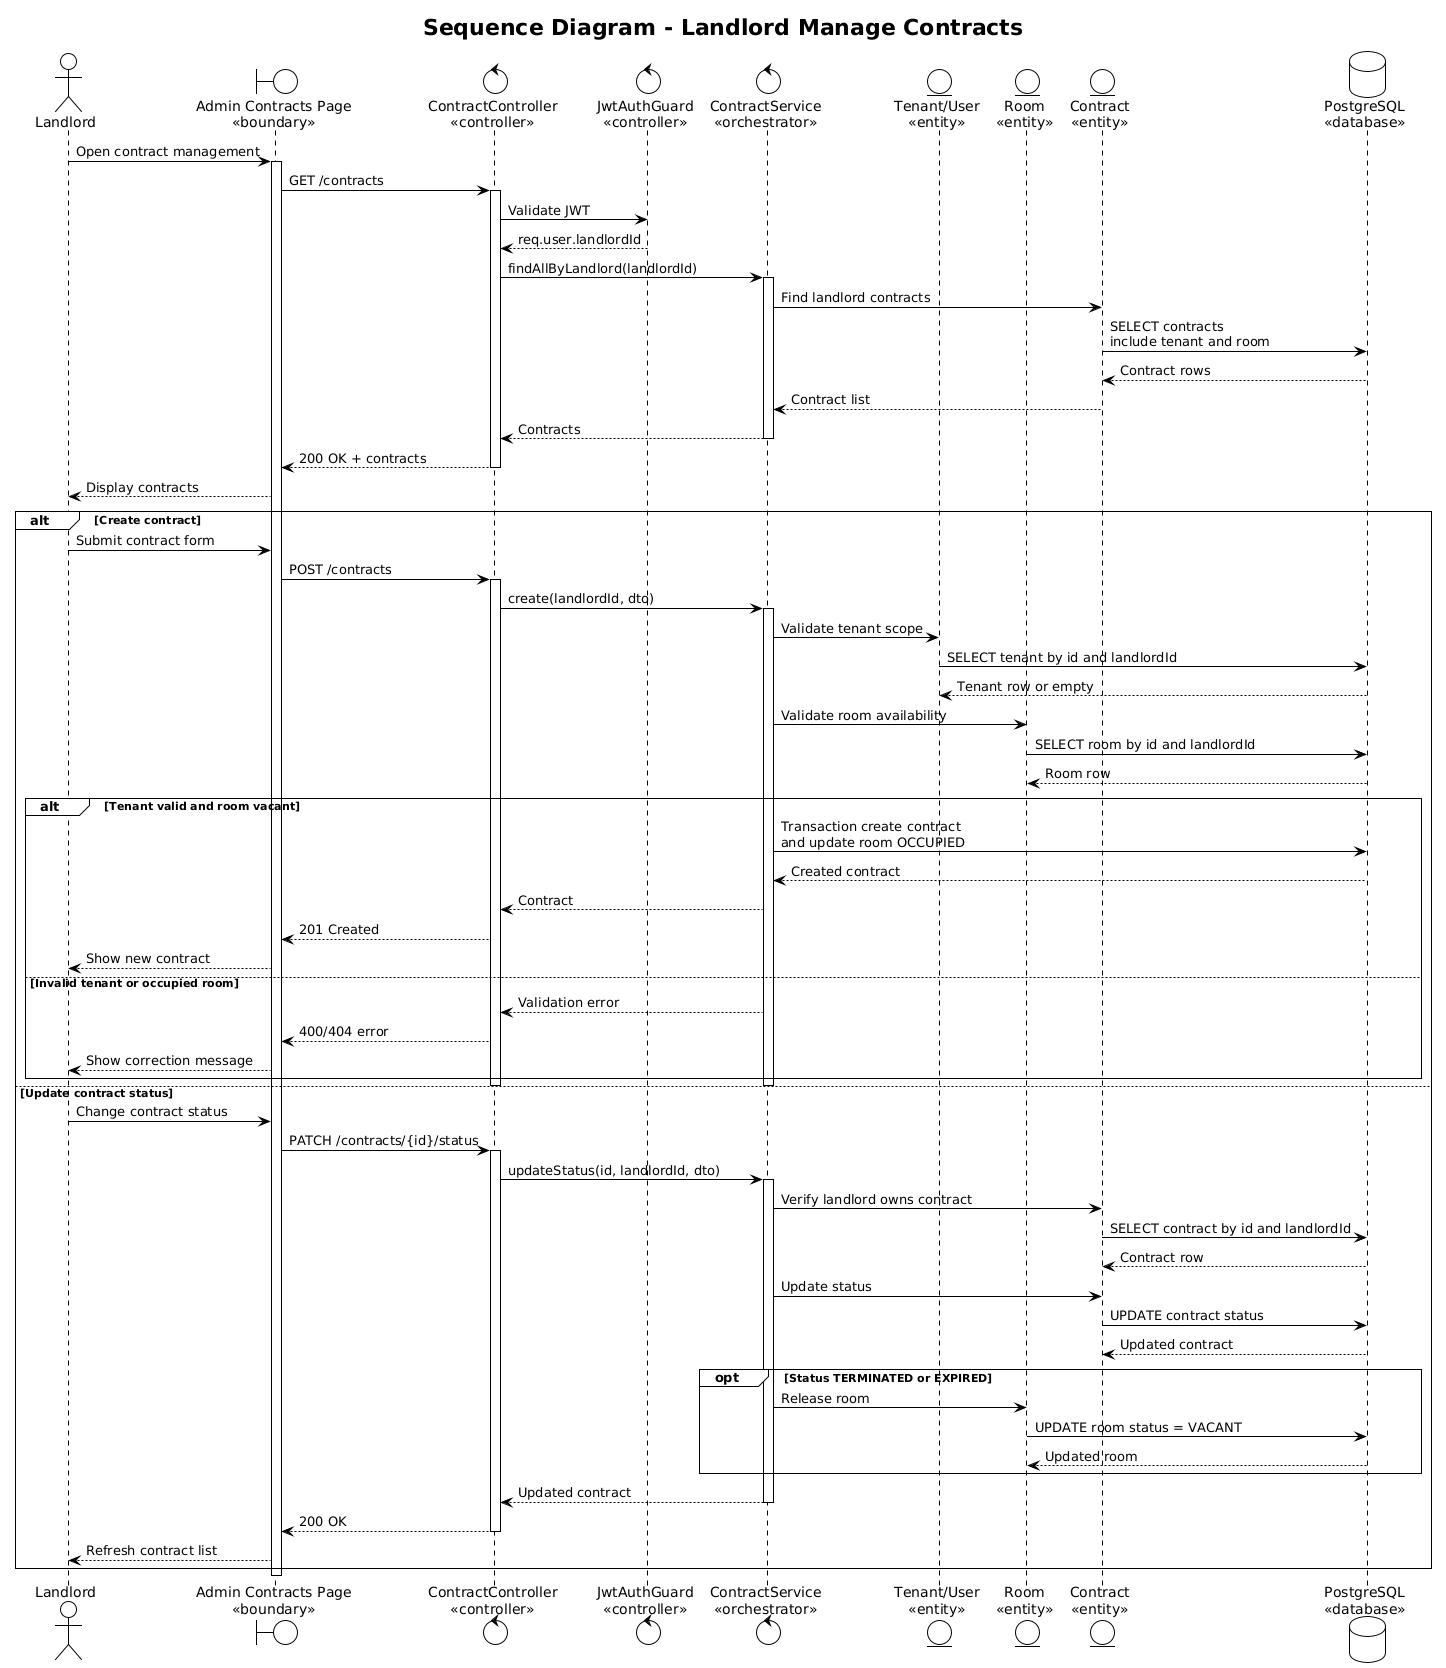
\includegraphics[width=0.9\textwidth]{seq_landlord_manage_contracts.png}
    \caption{Sequence Diagram - Manage Contracts}
    \label{fig:seq_landlord_manage_contracts}
\end{figure}

\subsubsection{Manage Invoices}
\textbf{Goal:} To create invoices, check payments, and export PDF bills.

\noindent \textbf{Primary Actor:} Landlord

\noindent \textbf{Pre-conditions:} The landlord is logged in, and an active contract exists.

\noindent \textbf{Main Success Scenario:}
\begin{enumerate}
    \item The landlord goes to the billing section.
    \item The landlord enters details like monthly price, electric usage, and water usage.
    \item The landlord saves the invoice.
    \item The system calculates the total amount, saves the invoice, and creates a PDF file.
    \item The landlord can view the PDF invoice with a VietQR code.
\end{enumerate}

\noindent \textbf{Alternative Flows:}
If the invoice details contain invalid values, the system returns an error.

\begin{figure}[H]
    \centering
    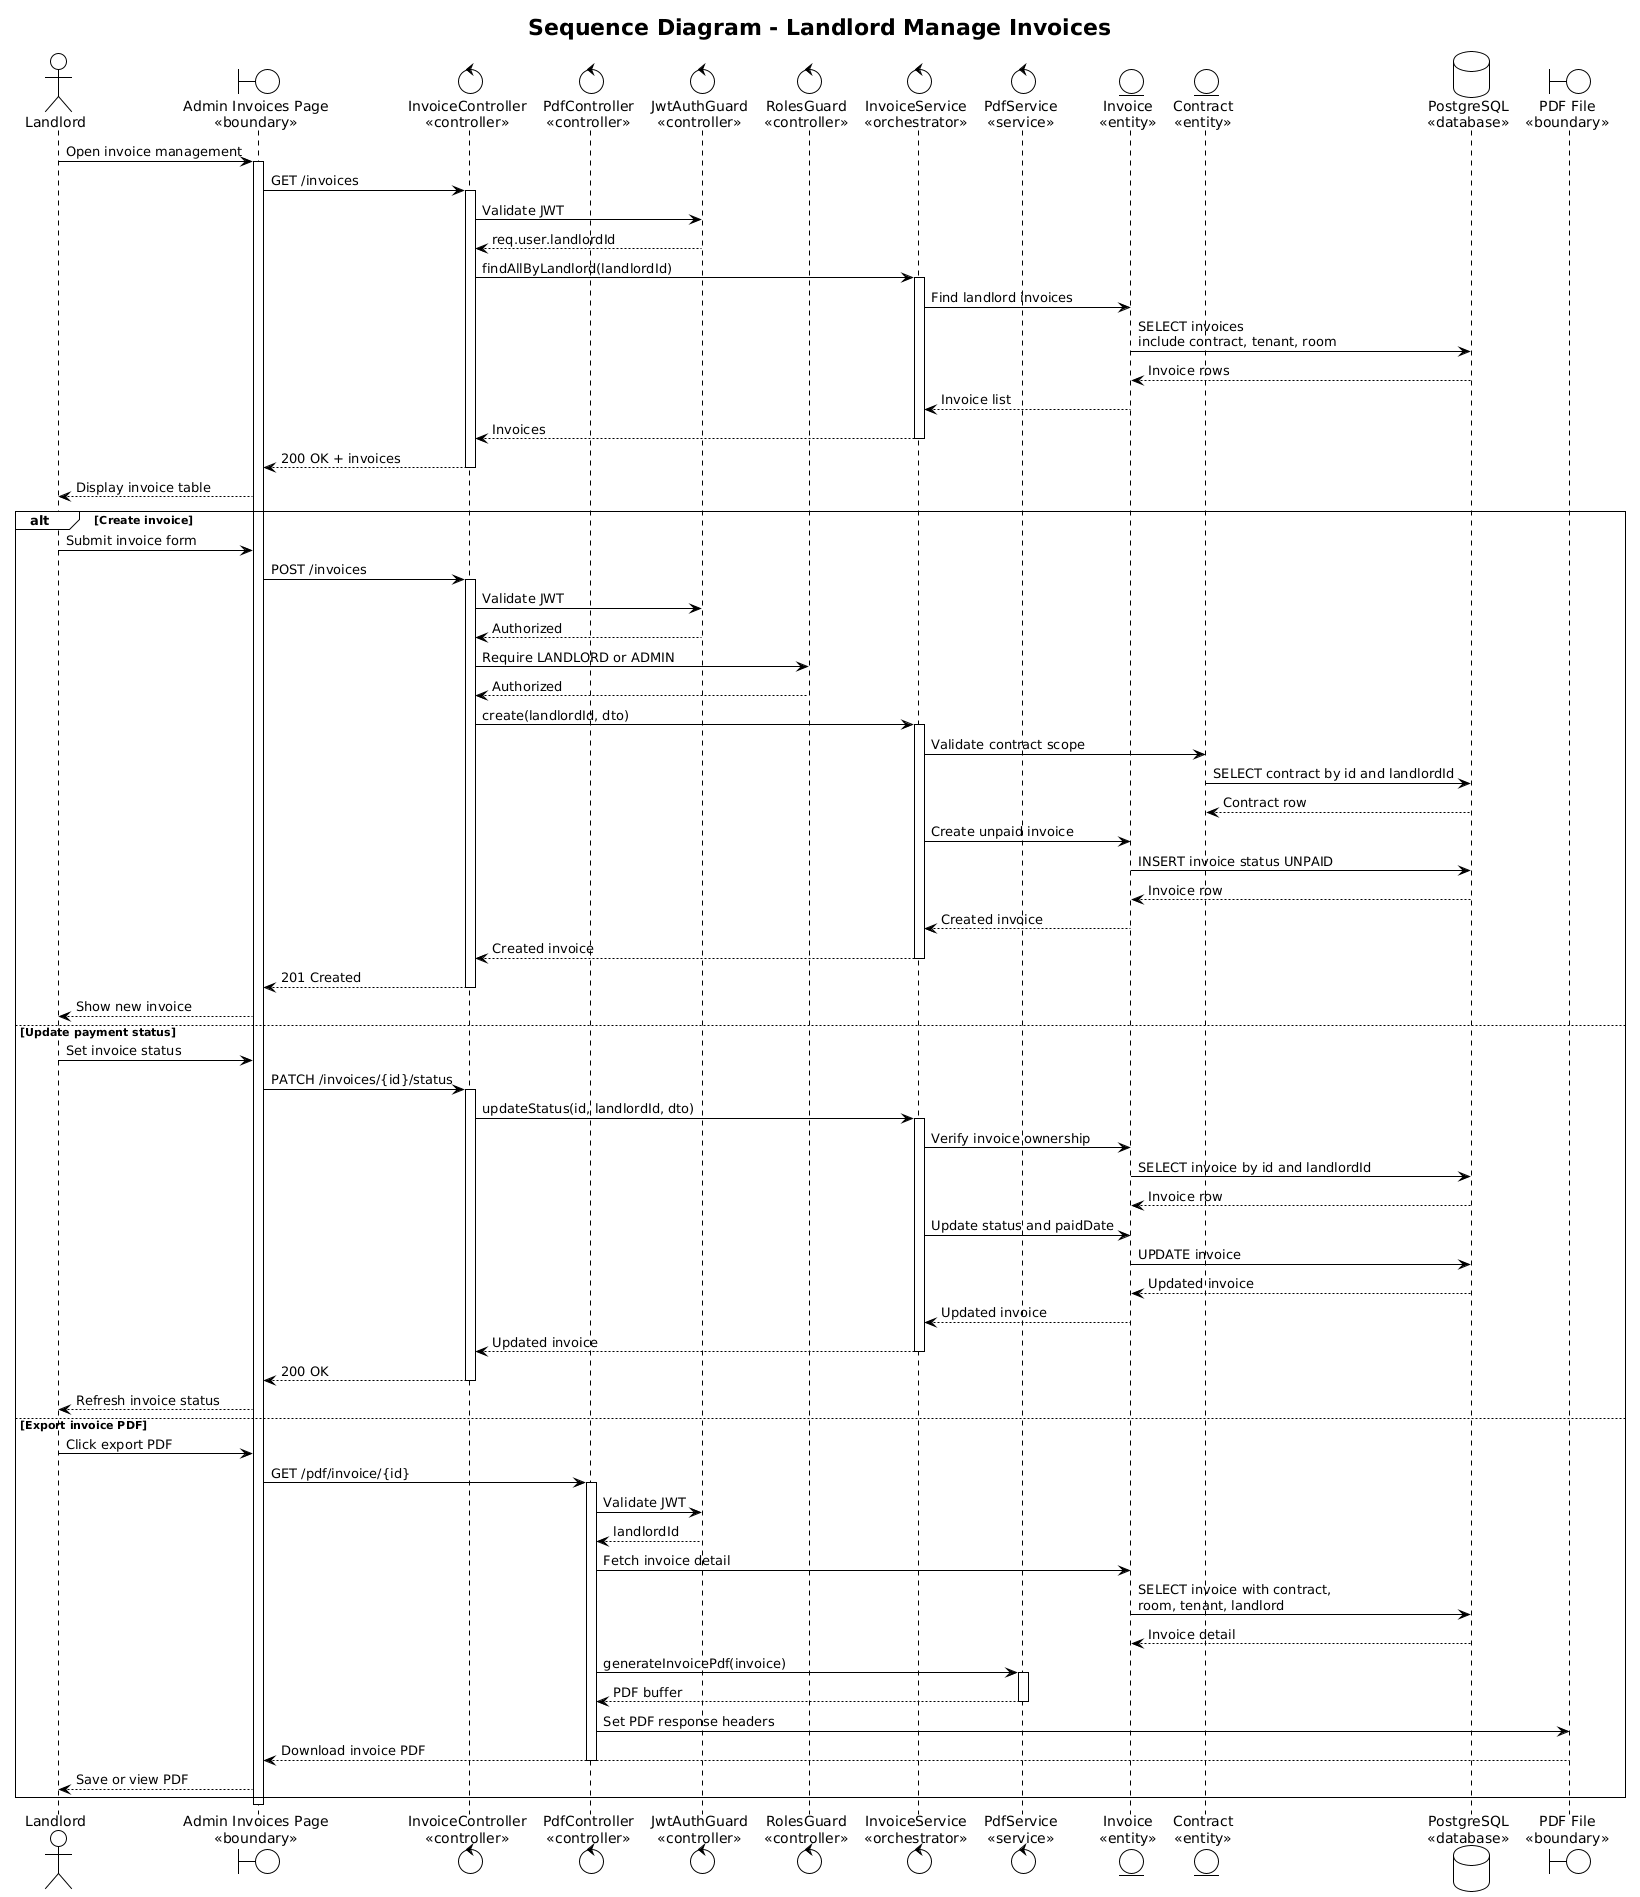
\includegraphics[width=0.9\textwidth]{seq_landlord_manage_invoices.png}
    \caption{Sequence Diagram - Manage Invoices}
    \label{fig:seq_landlord_manage_invoices}
\end{figure}

\subsubsection{Handle Incidents}
\textbf{Goal:} To review and solve tenant-reported incidents.

\noindent \textbf{Primary Actor:} Landlord

\noindent \textbf{Pre-conditions:} The landlord is logged in.

\noindent \textbf{Main Success Scenario:}
\begin{enumerate}
    \item The landlord opens the incident management list.
    \item The landlord reviews the pending issues reported by tenants.
    \item The landlord updates the incident status to "In Progress" or "Resolved".
    \item The system saves the status in the database and notifies the tenant in real time.
\end{enumerate}

\noindent \textbf{Alternative Flows:}
If the incident has already been resolved by another admin, the system prevents duplicate actions.

\begin{figure}[H]
    \centering
    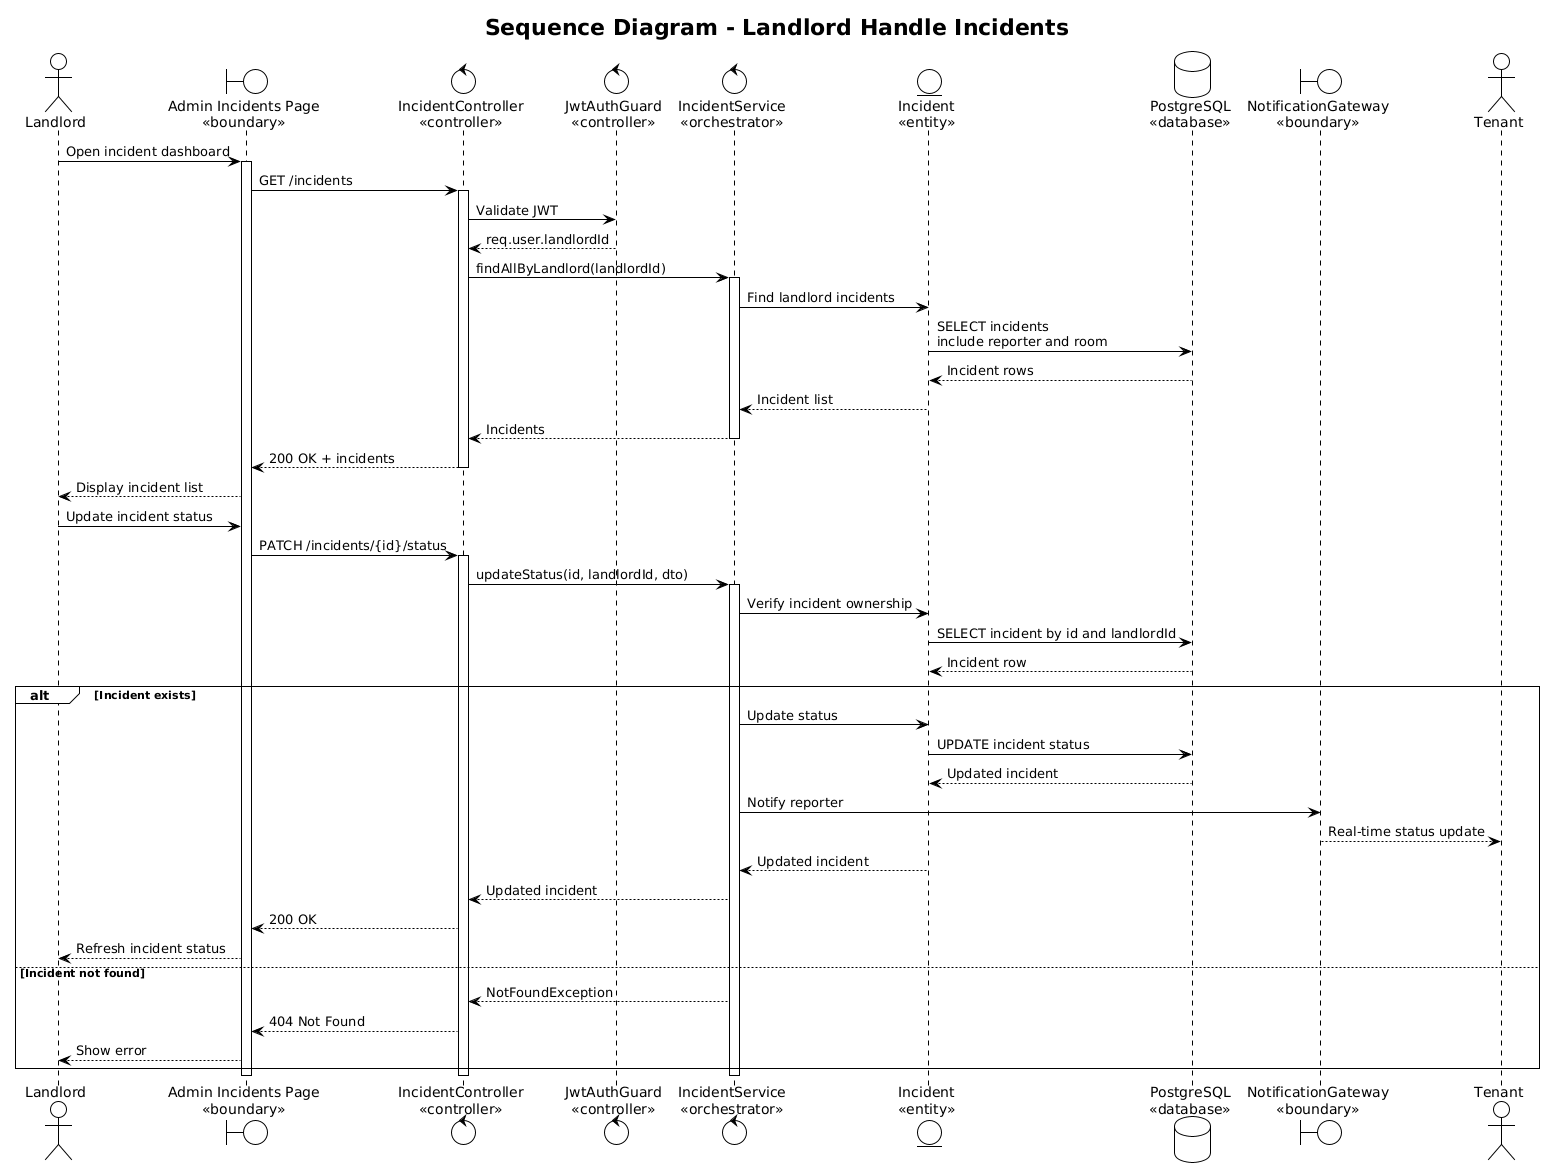
\includegraphics[width=0.9\textwidth]{seq_landlord_handle_incidents.png}
    \caption{Sequence Diagram - Handle Incidents}
    \label{fig:seq_landlord_handle_incidents}
\end{figure}

\subsubsection{Track Violations}
\textbf{Goal:} To record rules violations for tenants.

\noindent \textbf{Primary Actor:} Landlord

\noindent \textbf{Pre-conditions:} The landlord is logged in.

\noindent \textbf{Main Success Scenario:}
\begin{enumerate}
    \item The landlord opens the violations page.
    \item The landlord enters a description of a rule violation for a tenant.
    \item The landlord clicks "Add".
    \item The system saves the violation record and makes it visible to the tenant.
\end{enumerate}

\noindent \textbf{Alternative Flows:}
If the target tenant does not exist or has left, the system returns an error.

\begin{figure}[H]
    \centering
    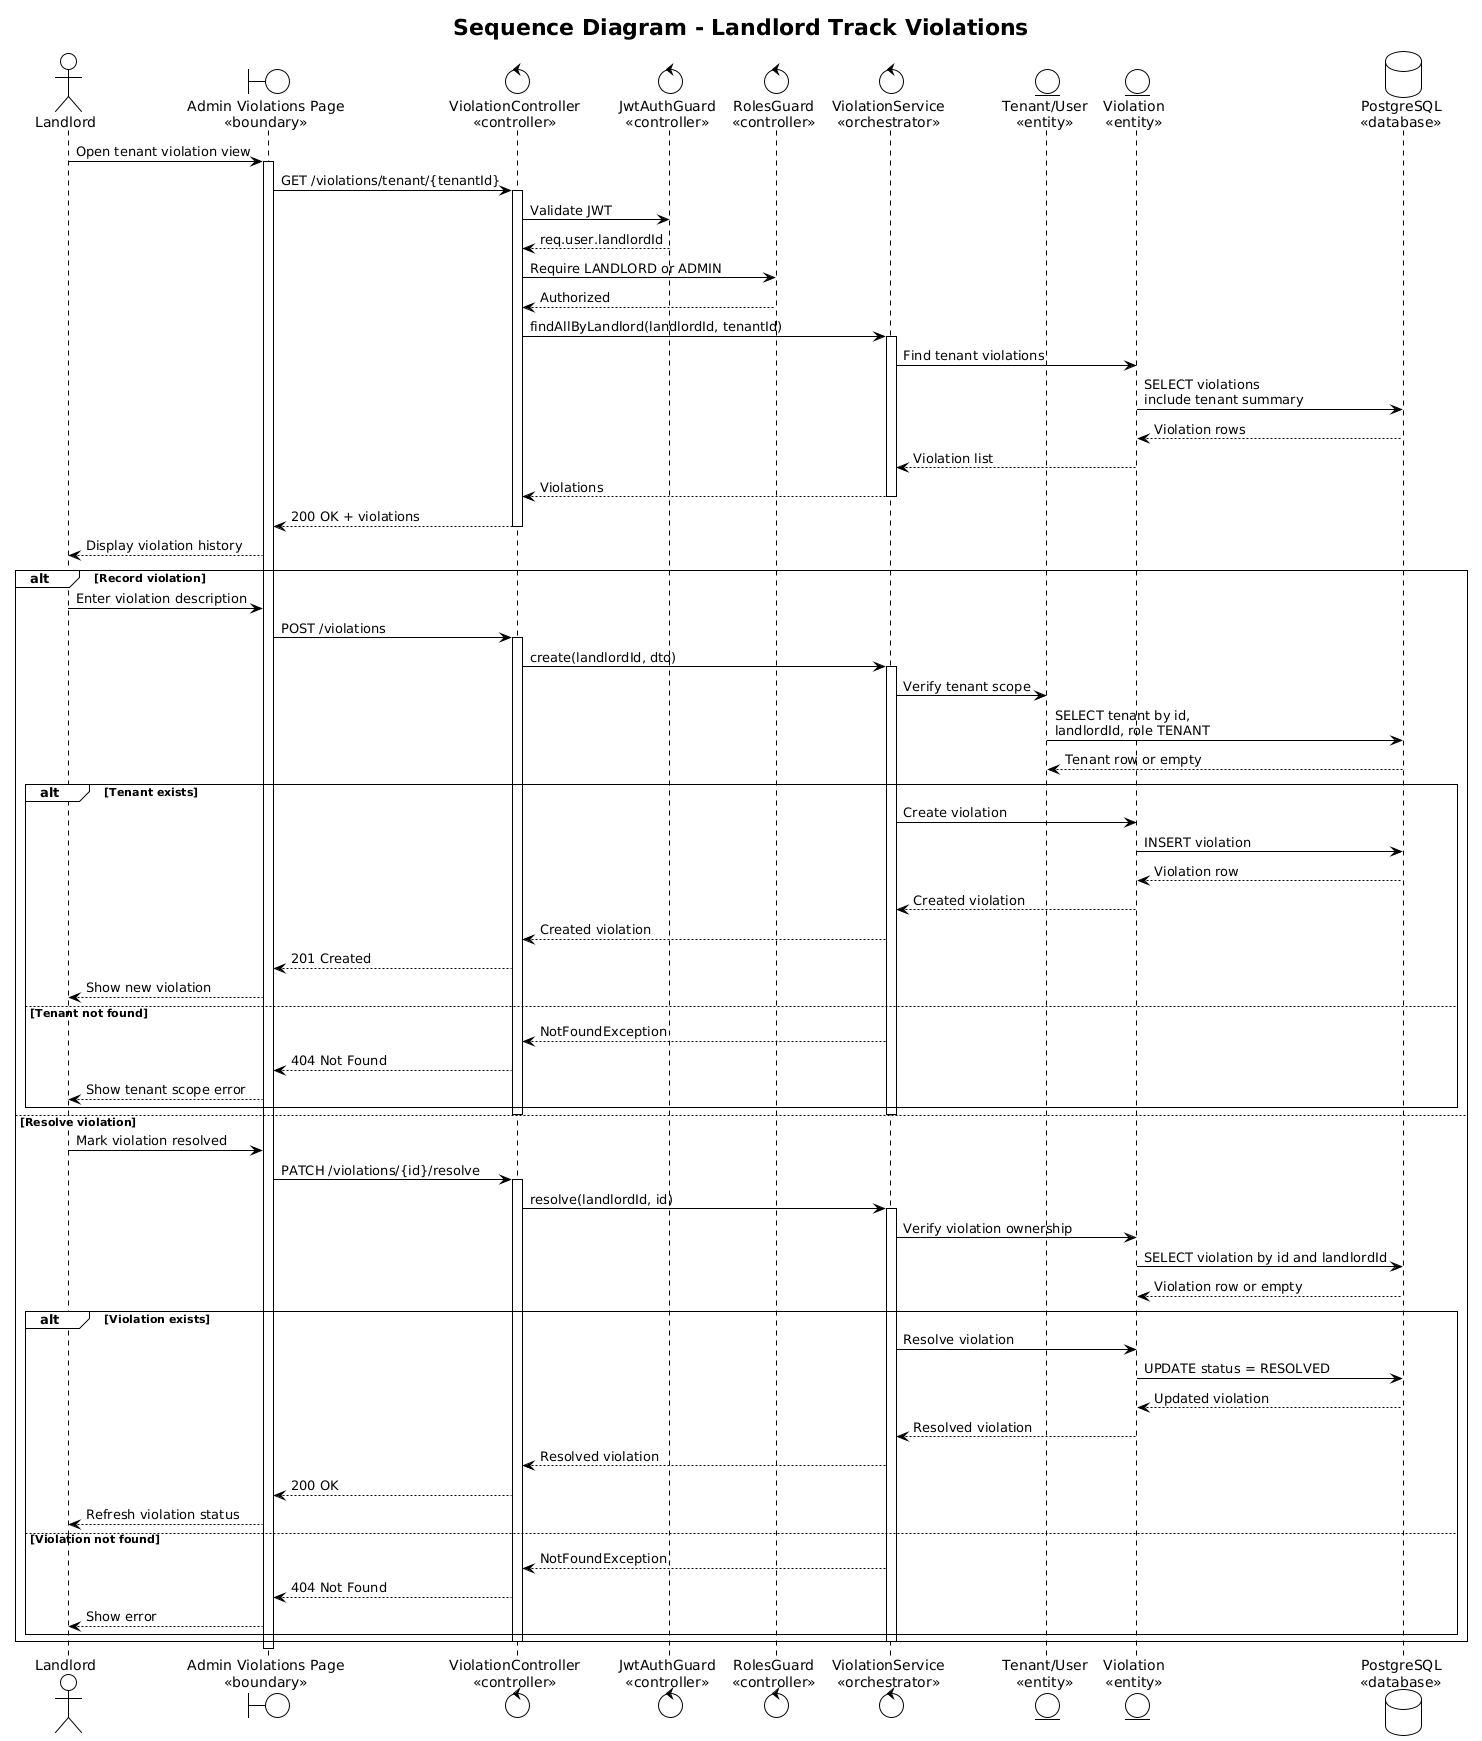
\includegraphics[width=0.9\textwidth]{seq_landlord_track_violations.png}
    \caption{Sequence Diagram - Track Violations}
    \label{fig:seq_landlord_track_violations}
\end{figure}


\section{Data Requirements}
The core database model uses a relational structure. The main entities are users, landlords, rooms, contracts, invoices, rent requests, incidents, and violations. Each record is scoped by a landlord identification code. This keeps the data private for each landlord. Main status fields include room availability, contract status, invoice payment status, user registration status, and incident resolution status.

\chapter{METHODOLOGY}

This chapter presents the architecture and implementation methods used to build the \textit{\textbf{Smart Boarding House Management System}}.

\section{Tools and Techniques}
Choosing the right tools is very important to build a reliable rental management platform. This section explains the technologies selected for the backend, frontend, supporting services, and system deployment, and the reasons for choosing them instead of other options.

\subsection{Backend Services}
For the backend, \textbf{NestJS} is chosen instead of simple frameworks like \textbf{Express}. \textbf{NestJS} provides a modular structure, dependency injection, and decorators, which makes it easy to organize the codebase. This organization is very helpful for implementing \textbf{Clean Architecture} and keeping the code neat as the system grows. \textbf{PostgreSQL} is used as the primary database because rental data like contracts and invoices must be secure and consistent. To connect the backend with \textbf{PostgreSQL}, \textbf{Prisma ORM} is used because it offers type-safe queries and makes database migrations easy. While \textbf{MongoDB} schemas are present in the codebase for potential logging development, the current active implementation relies entirely on \textbf{PostgreSQL} for data consistency.

\subsection{Frontend Portal}
For the frontend, \textbf{Next.js 14 App Router} is used instead of a standard \textbf{React} single-page application. \textbf{Next.js} offers server-side rendering, which is useful for the public landing page to load faster and have better search engine optimization. It also has a clean routing system that helps separate public pages, landlord admin pages, and the tenant portal. To manage the global application state, \textbf{Zustand} is chosen instead of \textbf{Redux}. \textbf{Zustand} is much lighter, has less boilerplate code, and is easier to learn, while still providing great performance for storing user sessions and UI states. For API requests, \textbf{Axios} is used with custom interceptors to automatically attach landlord identification headers and authorization tokens to every request.

\subsection{Supporting Services and Integrations}
To add special features to the platform, several supporting libraries and services are integrated. \textbf{Socket.IO} is used instead of constant HTTP polling to send notifications. This allows landlords to receive instant alerts when a tenant reports an incident or sends a room request. To store room images, \textbf{Cloudinary} is chosen instead of saving files locally on the server, which helps save disk space and automatically optimizes images for faster loading. For \textbf{AI} features, the \textbf{Google Generative AI} library with the \textbf{Gemini} model is used because it is very fast, accurate, and cost-effective for generating landlord notices and chatting with tenants. Finally, the \textbf{VietQR} image API is used to generate payment QR codes and insert them into invoice \textbf{PDF} files, allowing tenants to pay easily using their banking apps.

\subsection{Infrastructure and Deployment}
For deployment and production hosting, the system uses a serverless cloud infrastructure. The database is hosted on \textbf{Neon}, which provides a serverless \textbf{PostgreSQL} database. This allows the system to store rental data securely with high availability. The \textbf{NestJS} backend is deployed as a Web Service on \textbf{Render}. \textbf{Render} automatically builds the \textbf{NestJS} application from the backend directory and connects it to the \textbf{Neon} database. The \textbf{Next.js} frontend is deployed on \textbf{Vercel} because \textbf{Vercel} is optimized for \textbf{Next.js} applications, offering fast loading speeds. The frontend communicates with the backend on \textbf{Render} using environment variables. Both \textbf{Render} and \textbf{Vercel} are connected to the \textbf{GitHub} repository. This setup enables automatic \textbf{CI/CD} deployment, meaning any new code changes pushed to the repository are automatically built and deployed to the production environment.



\section{System Architecture}
This section describes how the different parts of the Smart Boarding House Management System are organized and connect with each other. The system is designed using a clean, layered structure to separate the user interface, business logic, and database operations.

\subsection{Overall System Structure}
The system follows a \textbf{client-server} architecture. The frontend is built with \textbf{Next.js} and acts as the client side. The backend is built with \textbf{NestJS} and acts as the server side. As shown in Figure \ref{fig:system_architecture}, the client and the server communicate using HTTP \textbf{REST APIs} for standard data requests and \textbf{Socket.IO} for real-time notifications. The backend server connects directly to the \textbf{PostgreSQL} database to read and store information. It also communicates with external services like \textbf{Cloudinary} to upload images, \textbf{Google Gemini} to run \textbf{AI} features, and the \textbf{VietQR API} to get payment codes.

\begin{figure}[H]
    \centering
    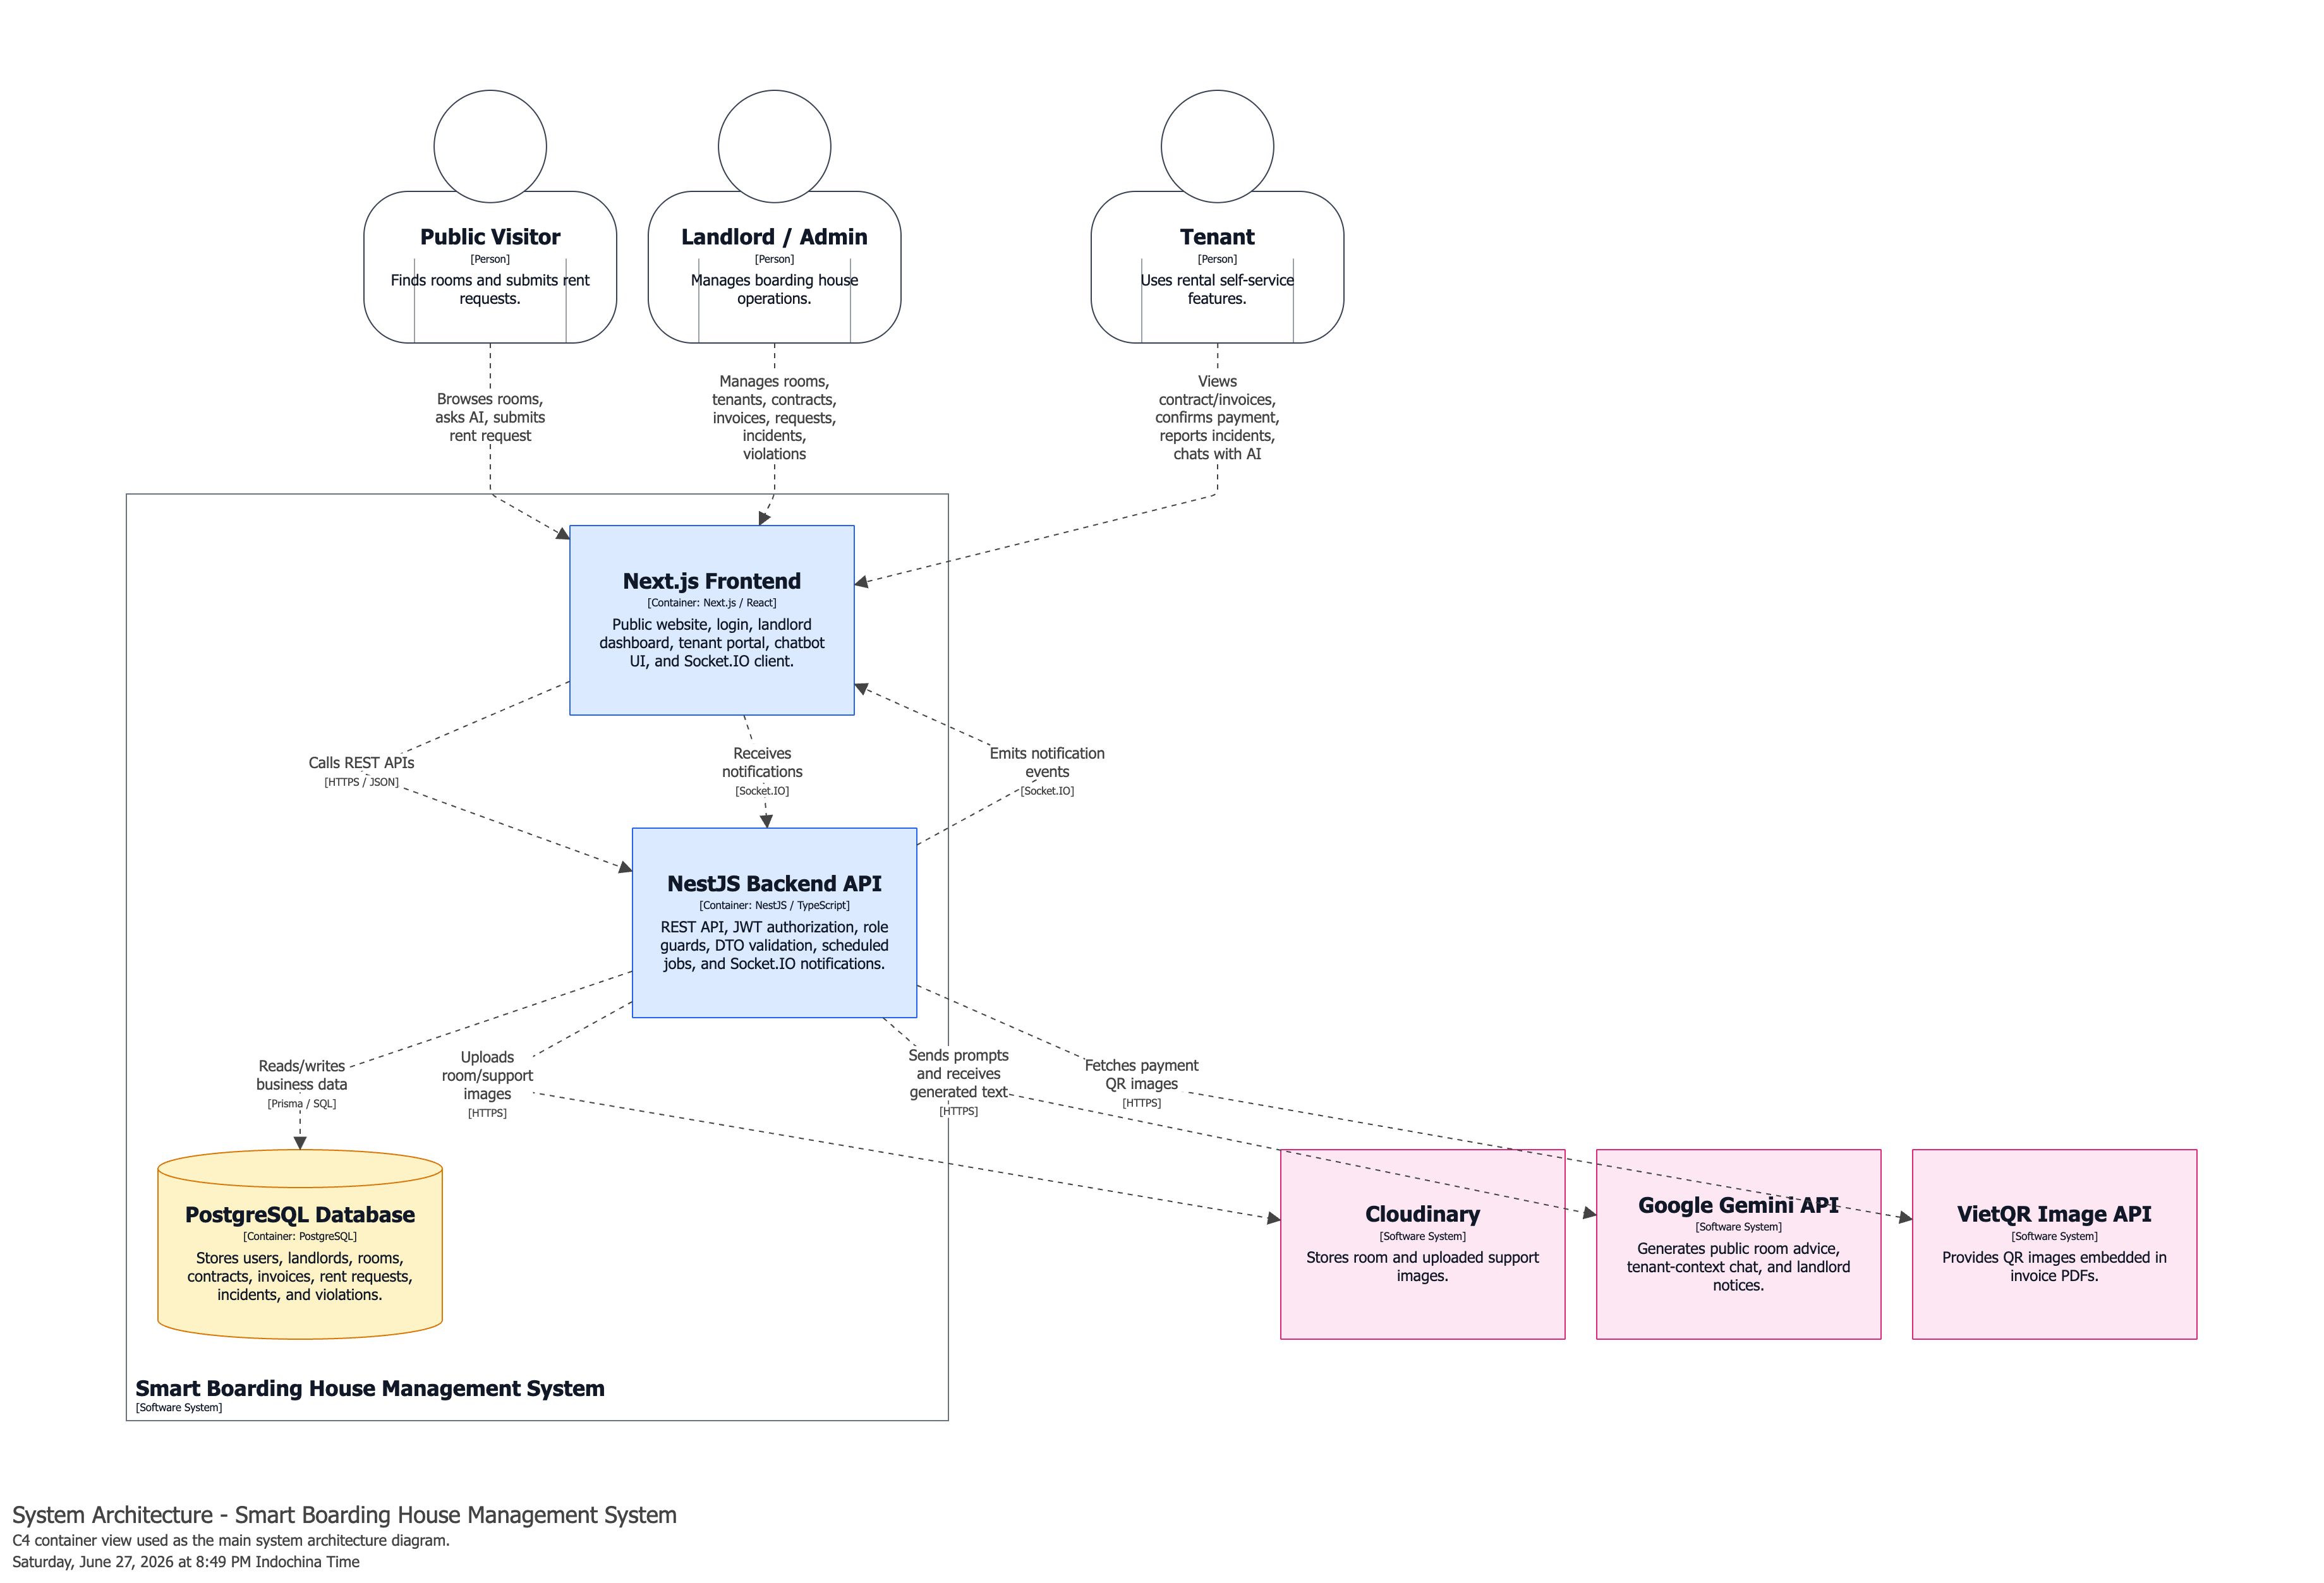
\includegraphics[width=1.0\textwidth]{SystemArchitecture.png}
    \caption{Overall System Architecture}
    \label{fig:system_architecture}
\end{figure}

\subsection{Layered Design}
To make the codebase easy to maintain, the \textbf{backend} and \textbf{frontend} are organized into three distinct layers: the \textbf{presentation layer}, the \textbf{application layer}, and the \textbf{infrastructure layer}.

The \textbf{presentation layer} is the top layer. In the \textbf{backend}, it contains HTTP controllers and data transfer objects to receive requests and send responses. In the \textbf{frontend}, it contains the visual pages and interactive components. The \textbf{presentation layer} does not process business rules; it only passes data to the next layer.

The \textbf{application layer} contains the core business logic of the system. For example, when a landlord creates a contract, the \textbf{application layer} checks if the room is vacant and updates the room status. It contains modules for authentication, room management, contract lifecycles, and invoice creation. This layer is completely independent of the database details or framework configurations.

The \textbf{infrastructure layer} is the bottom layer. It handles communication with external systems. In the \textbf{backend}, it includes database services to execute \textbf{PostgreSQL} queries using \textbf{Prisma}, and call external APIs like \textbf{Cloudinary} and \textbf{Google Generative AI}. This layered design ensures that changes in one part of the system, like upgrading the database, do not affect the rest of the application.


\section{Database Design}
The database is a very important part of the platform because it stores all information about rooms, tenants, contracts, and invoices. \textbf{PostgreSQL} is used as the database and \textbf{Prisma ORM} connects the backend server to it. This section explains the database structure, the relationships between different tables, and how the data is organized.

\subsection{Entity-Relationship Diagram}
To understand how the data is structured, an \textbf{Entity-Relationship Diagram (ERD)} is created. As shown in Figure \ref{fig:erd_diagram}, the database has eight main tables that represent the core parts of the boarding house system. These tables are \textbf{User}, \textbf{Landlord}, \textbf{Room}, \textbf{Contract}, \textbf{Invoice}, \textbf{RentRequest}, \textbf{Incident}, and \textbf{Violation}.

\begin{figure}[H]
    \centering
    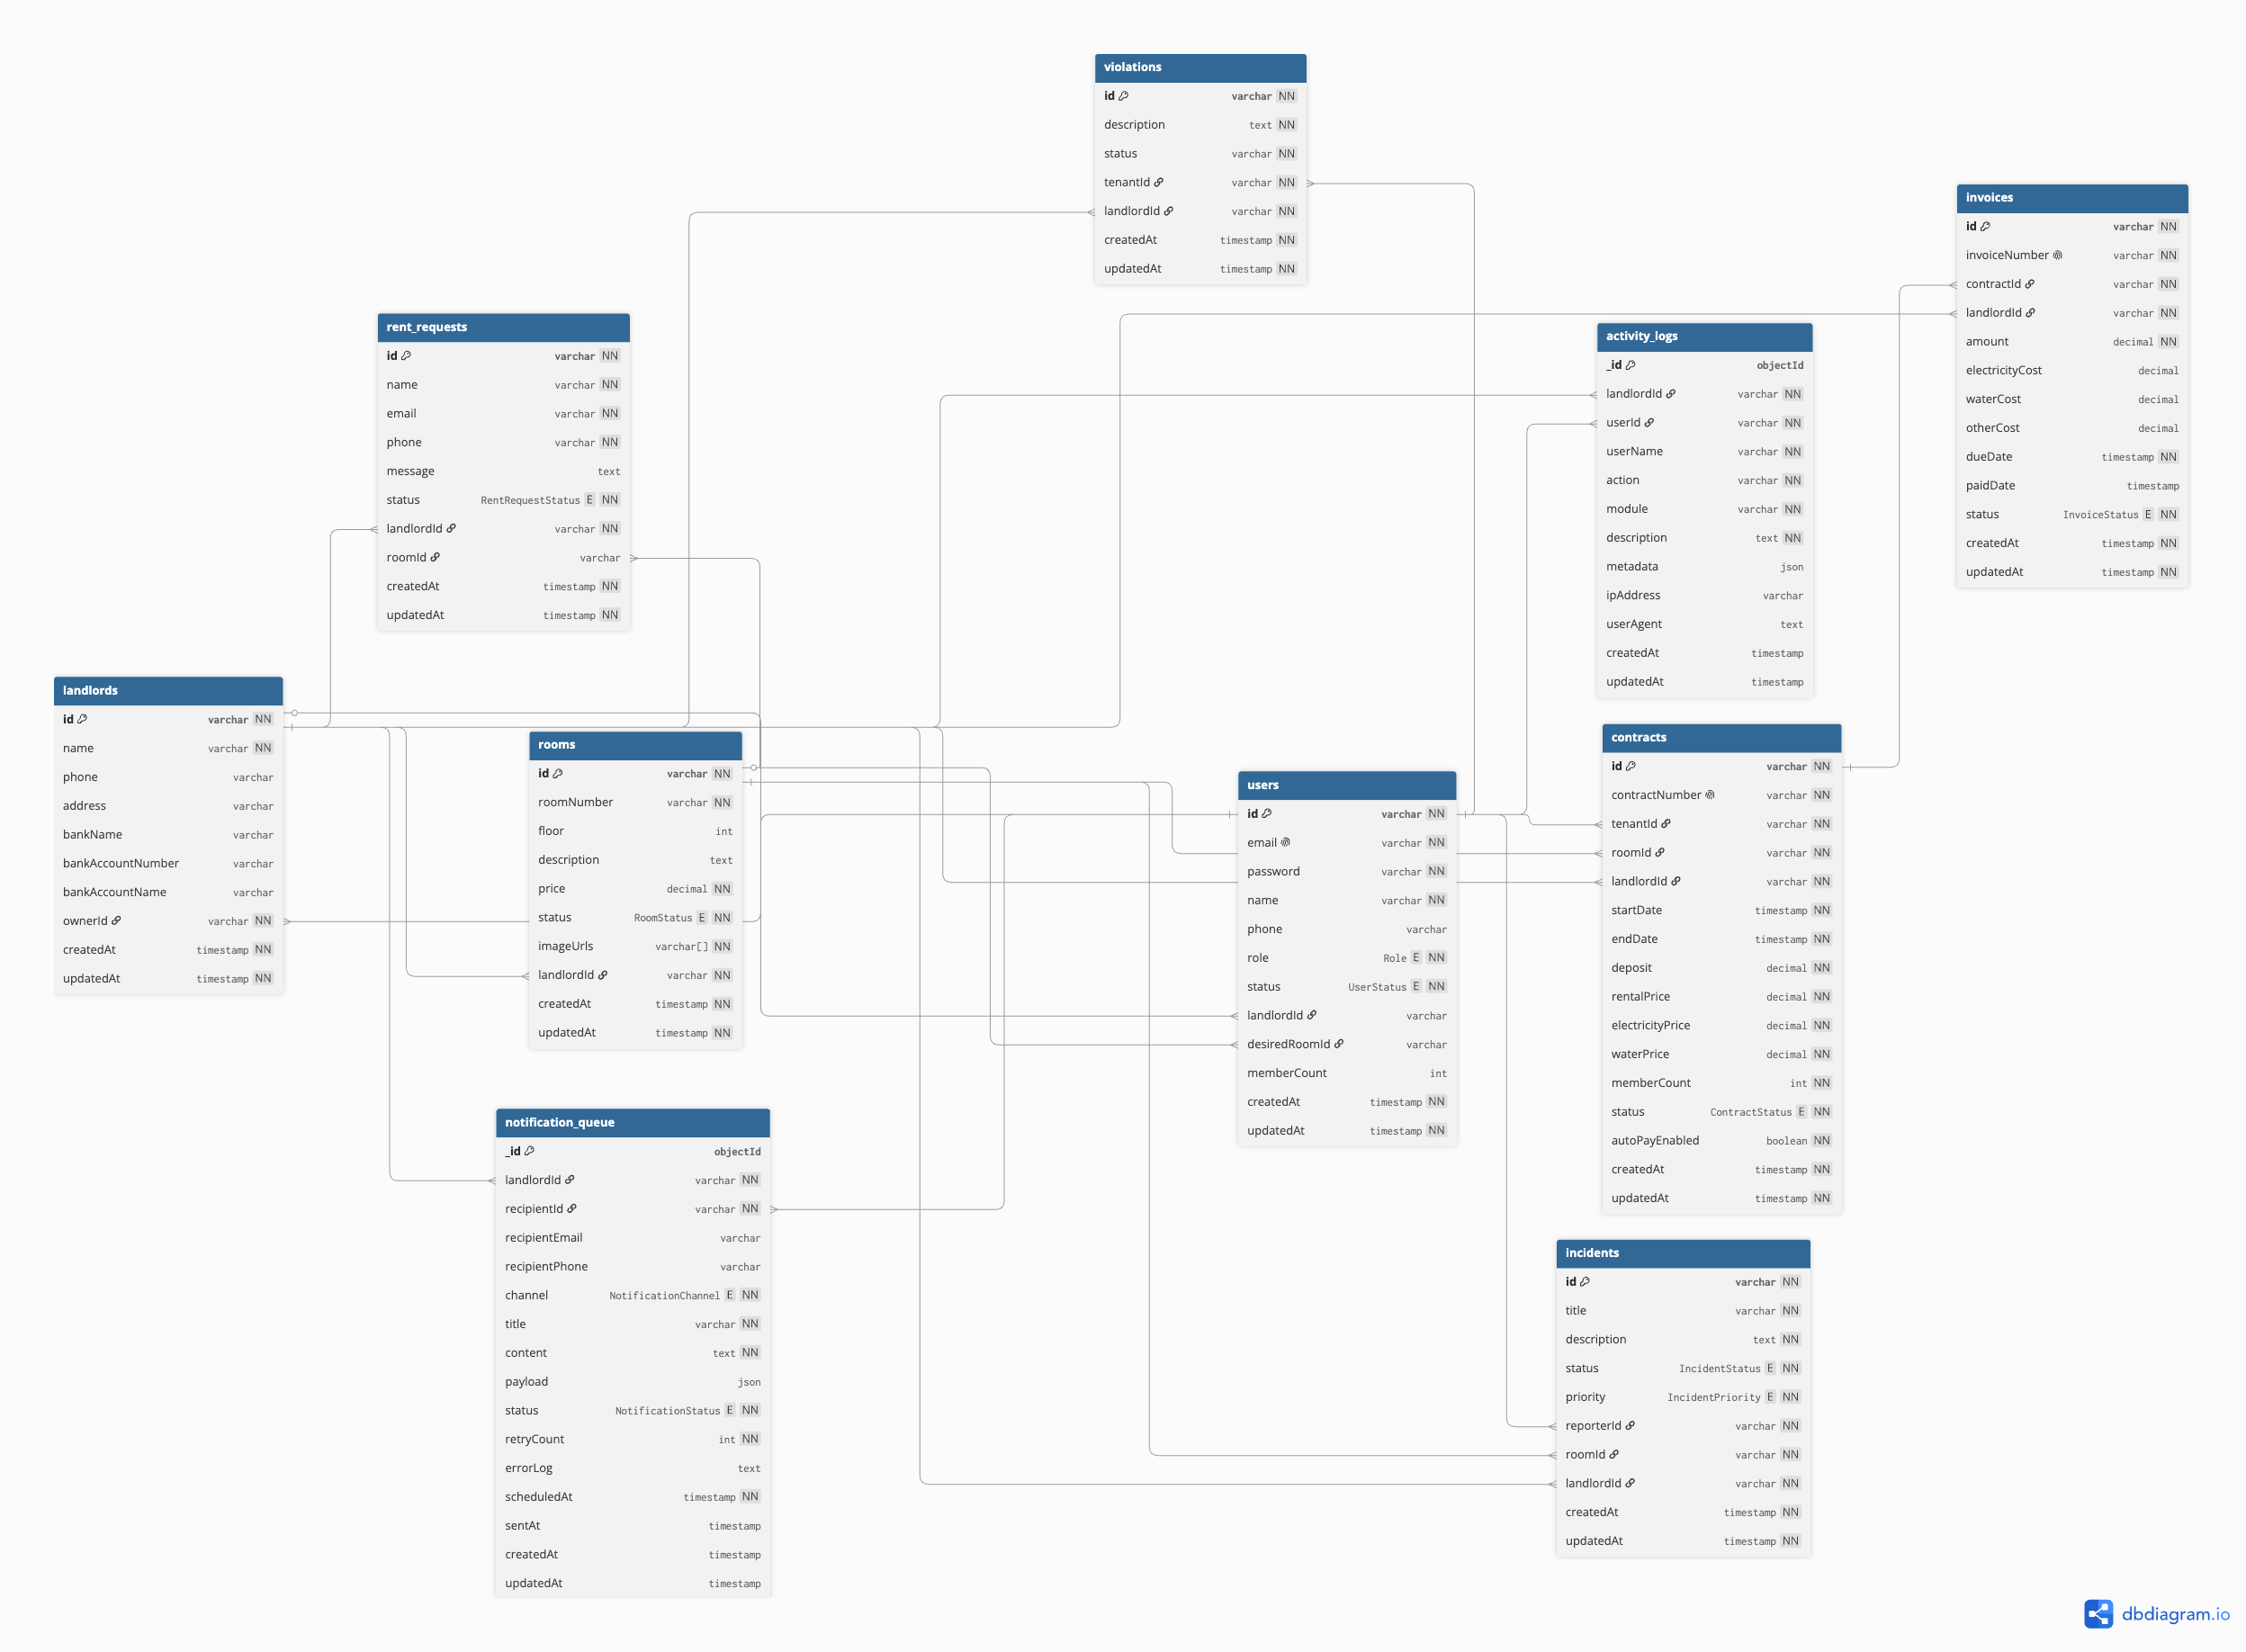
\includegraphics[width=1.0\textwidth]{erd.png}
    \caption{Database Entity-Relationship Diagram}
    \label{fig:erd_diagram}
\end{figure}

\subsection{Core Database Tables}
The \textbf{User} table stores information about all accounts in the system. Each user has an email, password, name, phone, status, and role (which can be \textbf{Admin}, \textbf{Landlord}, or \textbf{Tenant}). If the user is a tenant, they can also have a \textbf{landlordId} to connect them to a specific landlord.

The \textbf{Landlord} table stores the business profile of property owners. It contains details like the landlord's name, phone, address, and bank account information (bank name, account name, and account number). This bank information is used to generate \textbf{VietQR} codes on invoice \textbf{PDF}s automatically.

The \textbf{Room} table contains information about the rental rooms. Each room has a room number, floor, description, rental price, status (which can be \textbf{Vacant}, \textbf{Occupied}, or \textbf{Maintenance}), and a list of image URLs hosted on \textbf{Cloudinary}. Every room is connected to a specific landlord.

The \textbf{Contract} table represents the lease agreement. It connects a tenant user and a room together. It stores the start date, end date, deposit amount, monthly rental price, electricity price, water price, and status (which can be \textbf{Pending}, \textbf{Active}, \textbf{Expired}, or \textbf{Terminated}).

The \textbf{Invoice} table stores monthly billing records. It links to a specific contract and stores the total amount, electric cost, water cost, other costs, due date, payment date, and status (which can be \textbf{Unpaid}, \textbf{Paid}, \textbf{Overdue}, or \textbf{Cancelled}).

The \textbf{RentRequest} table stores requests from public visitors who want to ask about rooms. The \textbf{Incident} table stores repair and maintenance requests submitted by tenants. The \textbf{Violation} table stores rules violations recorded by landlords.

\subsection{Multi-Tenant Data Privacy}
To keep the data of each landlord private, the system uses a multi-tenant design. Most tables in the database, including \textbf{Room}, \textbf{Contract}, \textbf{Invoice}, \textbf{RentRequest}, \textbf{Incident}, and \textbf{Violation}, contain a \textbf{landlordId} field. When a landlord logs in, the \textbf{backend} server automatically filters all queries using their \textbf{landlordId}. This ensures that a landlord can only see their own rooms, contracts, and invoices, and cannot access data belonging to other landlords.


\section{Authentication and Authorization}
Security is a critical part of the Smart Boarding House Management System. The platform must ensure that only registered users can access private pages, and that landlords can only see their own rental data. To implement this, the backend uses token-based authentication and role-based access control.

\subsection{User Authentication with JWT}
The system uses JSON Web Tokens (JWT) to authenticate users. When a user logs in by entering their email and password, the authentication service validates their credentials. If the information is correct, the server generates a signed JWT token and returns it to the client. This token contains a payload with the user's identification code, email address, role, and landlord identification code. For every subsequent request, the client must send this token in the HTTP Authorization header as a Bearer token. To validate these tokens, the backend uses a NestJS Passport strategy. This strategy extracts the token, verifies its signature using a secret key, and automatically attaches the decoded user data to the request object as the authenticated user. The structure of this JWT token payload is described in Table \ref{tab:jwt_payload}.

\begin{table}[H]
    \centering
    \renewcommand{\arraystretch}{1.2}
    \begin{tabular}{|l|l|p{8cm}|}
        \hline
        \textbf{Claim Key} & \textbf{Data Type} & \textbf{Purpose and Description} \\
        \hline
        sub & String (UUID) & The unique identifier of the authenticated User. \\
        \hline
        email & String & The email address used to identify the user account. \\
        \hline
        role & Enum & The system role of the user (e.g., ADMIN, LANDLORD, or TENANT). \\
        \hline
        landlordId & String (UUID) & The landlord identifier used to filter data access for multi-tenancy. \\
        \hline
    \end{tabular}
    \caption{Structure of the JSON Web Token (JWT) Payload}
    \label{tab:jwt_payload}
\end{table}

\subsection{API Protection with Auth Guards}
To protect individual API endpoints, the backend implements custom NestJS guards. The primary guard is the JWT Auth Guard, which intercepts incoming requests to protected routes. If the request does not contain a valid token, the guard blocks the request and throws an unauthorized exception. For routes that require specific roles, the system combines the JWT Auth Guard with a Roles Guard. The Roles Guard uses a custom Roles decorator and the NestJS Reflector to read the roles allowed for a route. It checks the role of the logged-in user inside the request object and compares it with the required roles. For example, if a route is decorated for landlords only, a tenant attempting to access it will be blocked and receive a forbidden exception. The flowchart in Figure \ref{fig:auth_guard_flowchart} shows how requests are processed through these guards.

\begin{figure}[H]
    \centering
    \begin{tikzpicture}[scale=0.9, every node/.style={transform shape}]
        \draw[fill=blue!10, draw=blue!50, rounded corners] (0,0) rectangle (2.8,1.2) node[pos=.5, align=center] {Client Request \\ (Bearer Token)};
        \draw[->, thick] (2.8,0.6) -- (3.6,0.6);
        \draw[fill=blue!10, draw=blue!50, rounded corners] (3.6,0) rectangle (6.6,1.2) node[pos=.5, align=center] {JWT Auth Guard \\ (Token Validation)};
        \draw[->, thick] (6.6,0.6) -- (7.4,0.6);
        \draw[fill=blue!10, draw=blue!50, rounded corners] (7.4,0) rectangle (10.4,1.2) node[pos=.5, align=center] {Roles Guard \\ (Role Checking)};
        \draw[->, thick] (10.4,0.6) -- (11.2,0.6);
        \draw[fill=green!10, draw=green!50, rounded corners] (11.2,0) rectangle (14.2,1.2) node[pos=.5, align=center] {Route Controller \\ (Resource Access)};
        
        \draw[->, thick] (5.1,0) -- (5.1,-1);
        \draw[fill=red!10, draw=red!50, rounded corners] (3.6,-2.2) rectangle (6.6,-1) node[pos=.5, align=center] {Unauthorized \\ (API Blocked)};
        
        \draw[->, thick] (8.9,0) -- (8.9,-1);
        \draw[fill=red!10, draw=red!50, rounded corners] (7.4,-2.2) rectangle (10.4,-1) node[pos=.5, align=center] {Forbidden \\ (Access Blocked)};
    \end{tikzpicture}
    \caption{Authentication and Authorization Guard Flowchart}
    \label{fig:auth_guard_flowchart}
\end{figure}

\subsection{Multi-Tenant Authorization Filter}
Apart from roles, the system enforces multi-tenant authorization using the landlord identification code. Because multiple landlords share the same database, the \textbf{backend} must prevent cross-tenant access. During authentication, the landlord's unique identification code is stored inside the \textbf{JWT} token. When a landlord requests room listings, contracts, or invoice records, the corresponding backend service reads this \textbf{landlordId} code directly from the request user object. The database query then filters the results based on this code. This technique guarantees that landlords can never view or modify the records of other property owners, even if they try to bypass the frontend interface.



\section{Automation and Business Logic}
This section describes the technical implementation of key business processes in the \textbf{backend}. To ensure data consistency and provide a good user experience, the system automates several workflows using database transactions, real-time messaging, and scheduled background tasks. These automated tasks include contract expiration checks, which run daily to return rooms to vacant status when leases end, and startup consistency checks, which automatically fix any room marked occupied that lacks an active contract.

\subsection{Rental Contract Creation}
Creating a new rental contract requires updating multiple records at the same time. As shown in the activity diagram (Figure \ref{fig:activity_create_contract}), when a landlord creates a contract, the system must verify room availability, save the contract details, and update the room status to occupied. To implement this safely, the \textbf{NestJS} backend uses a \textbf{Prisma} database transaction. This transaction guarantees that if any step fails (for example, if the tenant is invalid), the database rolls back to its previous state. This prevents bugs where a contract is created but the room remains vacant, or a room is marked occupied without an active contract.

\begin{figure}[H]
    \centering
    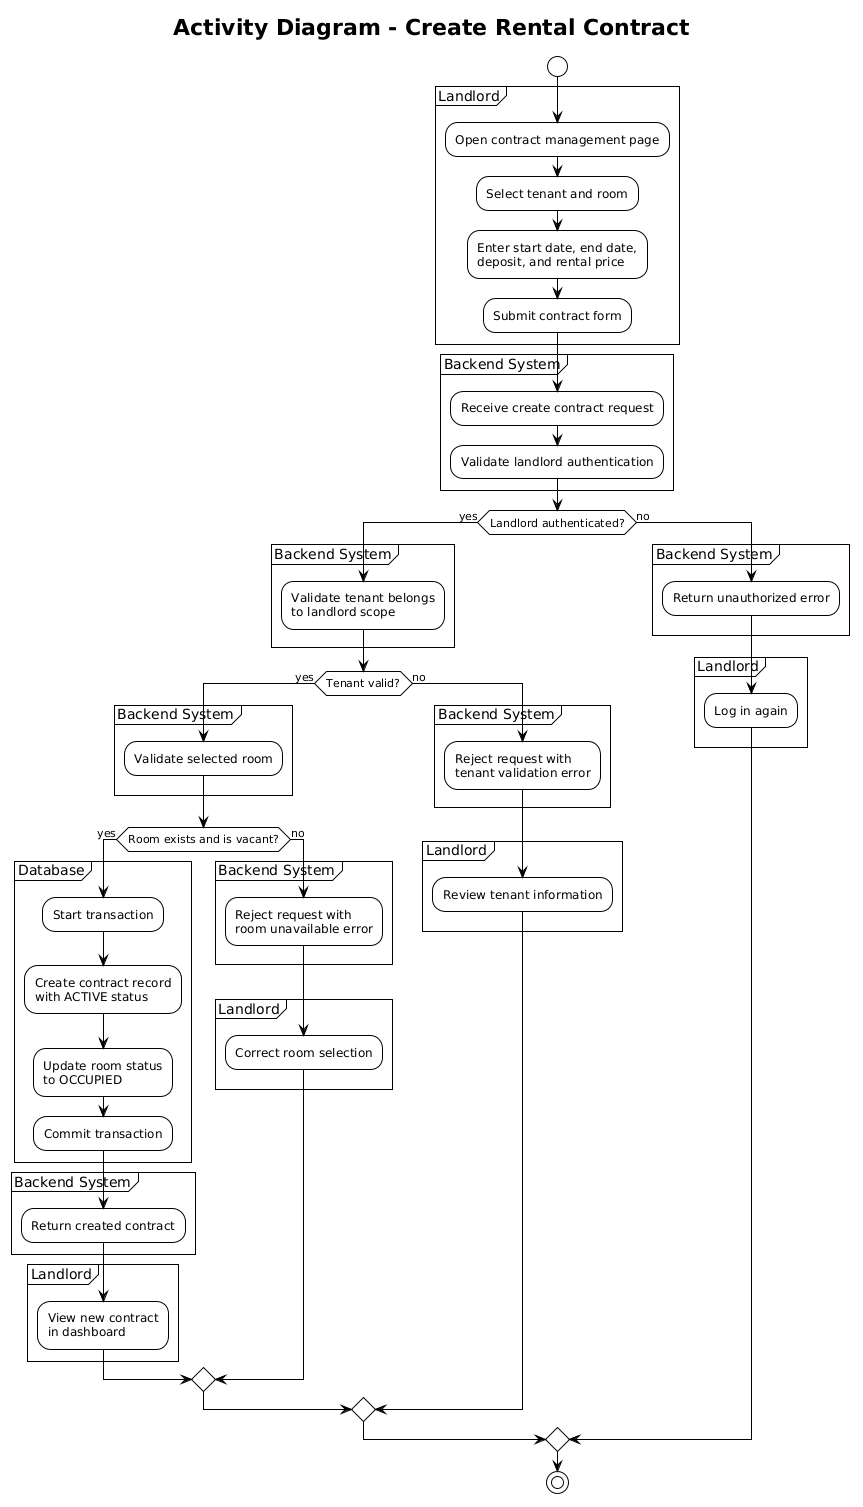
\includegraphics[width=0.75\textwidth]{activity_create_contract.png}
    \caption{Activity Diagram - Contract Creation Process}
    \label{fig:activity_create_contract}
\end{figure}

\subsection{Invoice Payment and Verification}
The monthly billing cycle is managed through automated invoice generation and a structured payment verification flow. At the beginning of each month, a \textbf{NestJS} cron job runs automatically to create unpaid invoices for all active contracts. As shown in the activity diagram (Figure \ref{fig:activity_invoice_payment_verification}), once an invoice is created, the tenant can view it and scan the generated \textbf{VietQR} code to make a bank transfer. After transferring the money, the tenant marks the invoice as paid in the portal, which immediately changes its status to \textbf{Paid} and records the payment timestamp. The backend simultaneously broadcasts a real-time \textbf{Socket.IO} notification to the landlord's dashboard. The landlord can then manually verify the bank transfer and, if necessary, adjust the invoice status through the administration panel.

\begin{figure}[H]
    \centering
    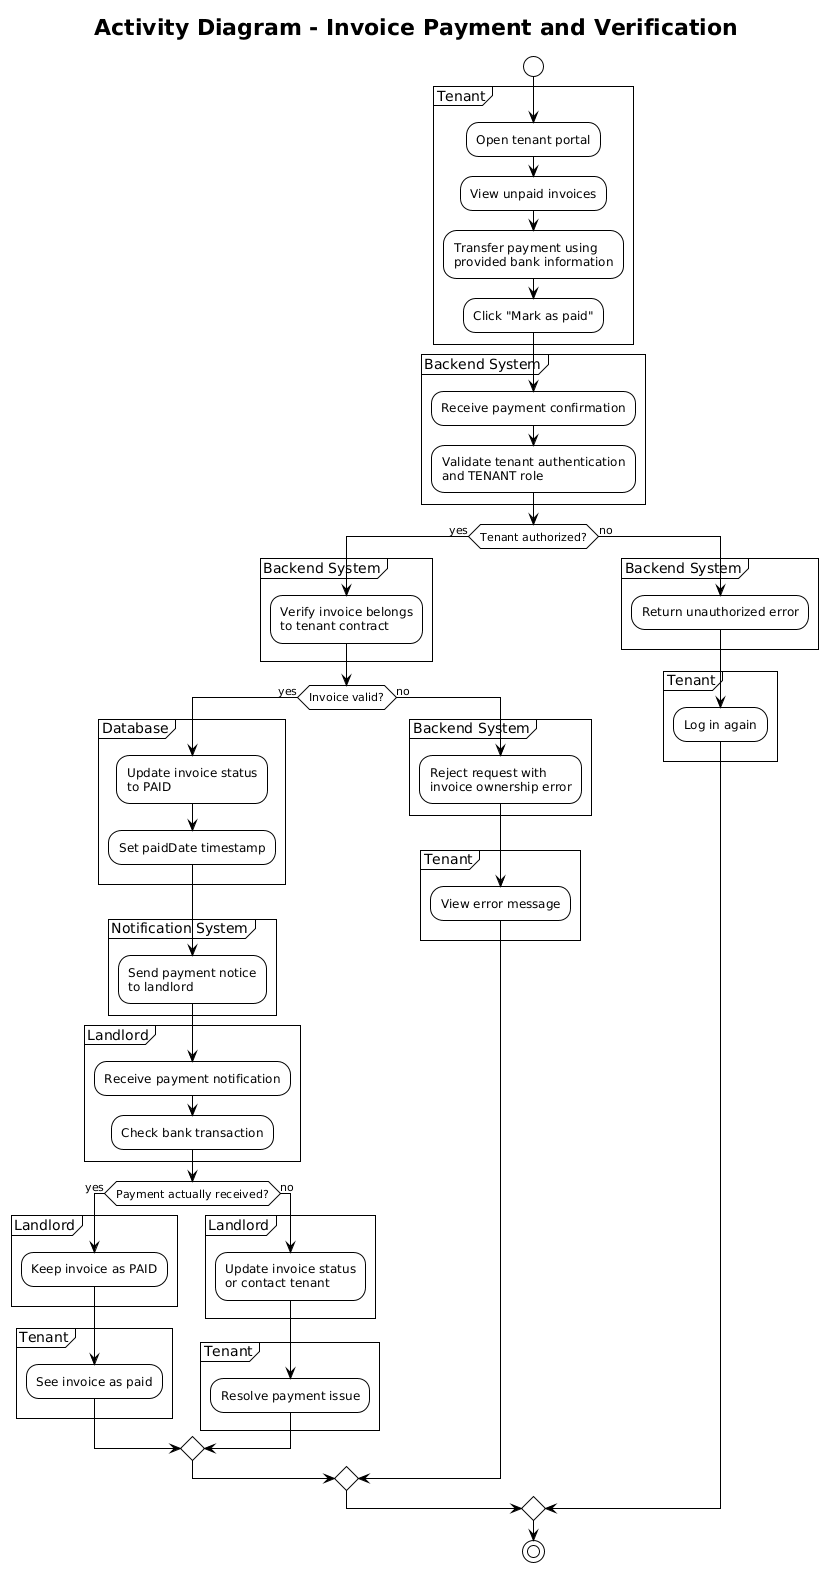
\includegraphics[width=0.75\textwidth]{activity_invoice_payment_verification.png}
    \caption{Activity Diagram - Invoice Payment and Verification}
    \label{fig:activity_invoice_payment_verification}
\end{figure}

\subsection{Tenant Incident Handling}
Managing room repairs quickly requires close cooperation between tenants and landlords. As shown in the activity diagram (Figure \ref{fig:activity_tenant_incident_handling}), the process starts when a tenant submits a new incident report with a priority level. The \textbf{backend} saves the incident in the database with a pending status and immediately broadcasts a \textbf{WebSocket} event to the landlord's dashboard using \textbf{Socket.IO}. The landlord reviews the incident, assigns a technician, and updates the status to in-progress. Once the issue is fixed, the landlord marks it as resolved. The system updates the status in the database and sends a real-time message back to the tenant's portal to notify them.

\begin{figure}[H]
    \centering
    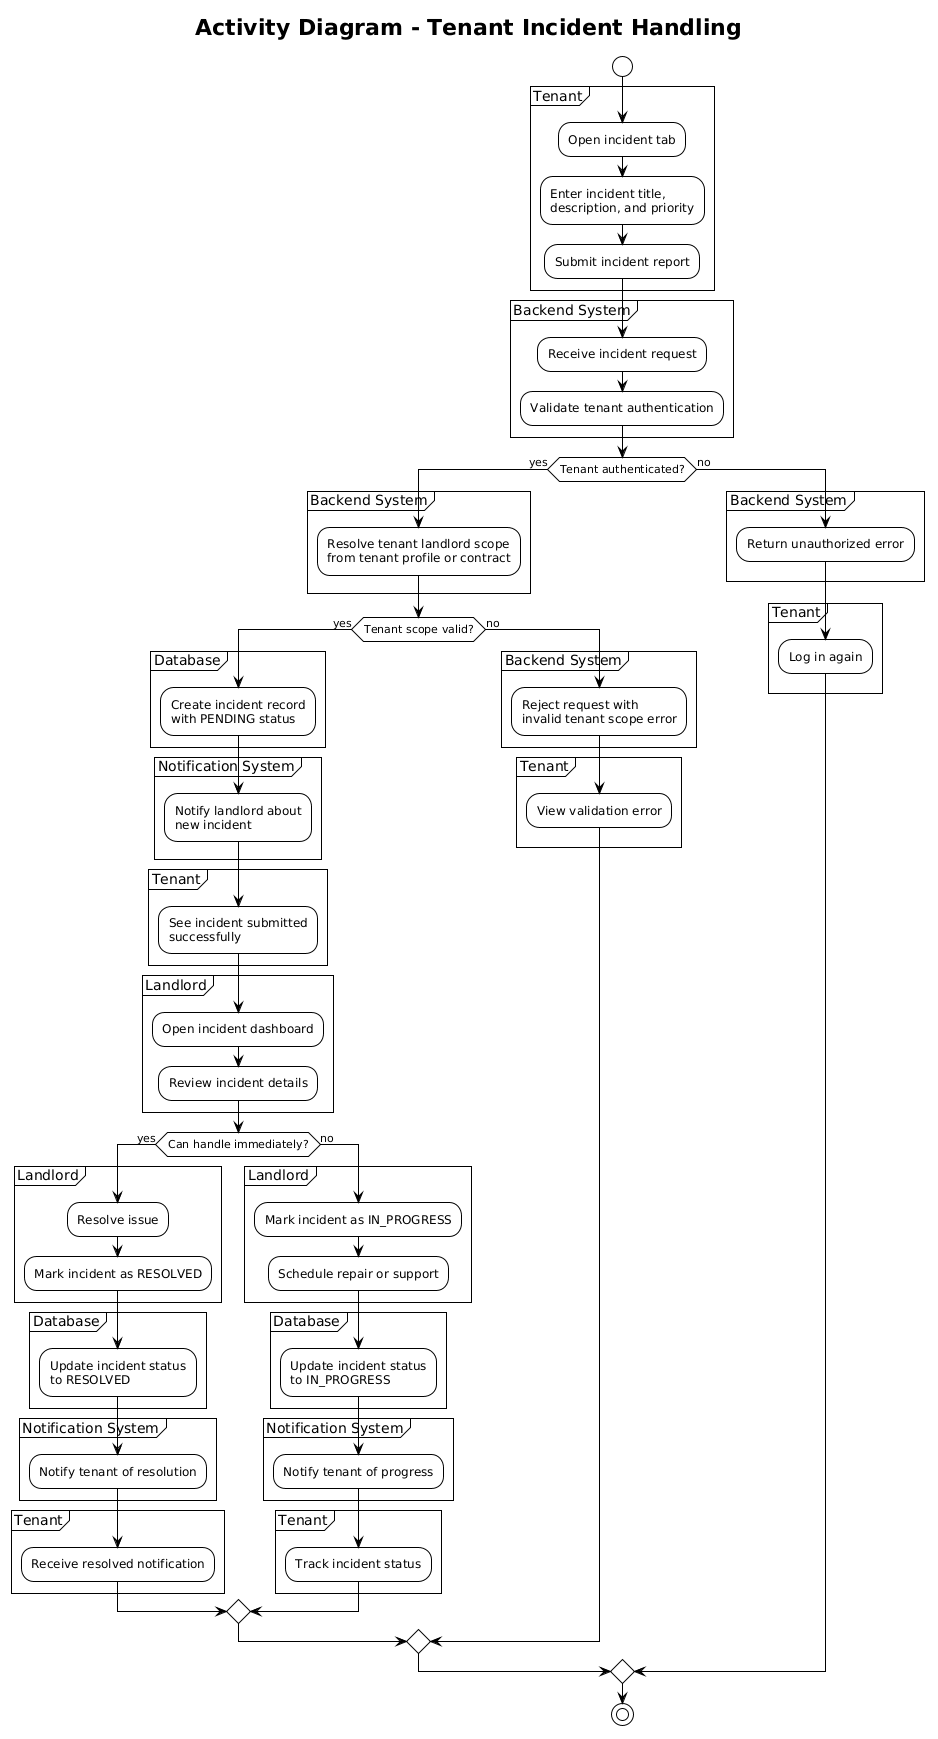
\includegraphics[width=0.75\textwidth]{activity_tenant_incident_handling.png}
    \caption{Activity Diagram - Tenant Incident Handling}
    \label{fig:activity_tenant_incident_handling}
\end{figure}


\section{AI Integration}
The platform integrates advanced artificial intelligence and optical character recognition to automate administrative workflows and improve communication. This section describes how the AI assistant and the OCR utility meter reader are built and how they process data.

\subsection{AI Assistant with Google Gemini}
The \textbf{AI} service is built using the official \textbf{Google Generative AI} library and the \textbf{Gemini 3.1 Flash Lite} model. This model was chosen because it provides fast responses and is highly accurate for text processing. The system implements three distinct assistant modes to help different users, as summarized in Table \ref{tab:ai_modes}.

\begin{table}[H]
    \centering
    \renewcommand{\arraystretch}{1.2}
    \begin{tabular}{|p{3cm}|p{3.5cm}|p{6.5cm}|}
        \hline
        \textbf{Assistant Mode} & \textbf{Database Context Injected} & \textbf{Core Capability} \\
        \hline
        Notice Generator & None (Direct prompt input) & Generates polite, formal boarding house announcements in Vietnamese. \\
        \hline
        RentBot (Public) & Room number, rental price, floor, status, description. & Answers visitor questions about vacant rooms and directs them to register. \\
        \hline
        Tenant Assistant & Contract dates, monthly rent, deposits, unpaid invoices, violations, incidents. & Provides personalized rental Q\&A, checks bills, and explains rules. \\
        \hline
    \end{tabular}
    \caption{Comparison of AI Assistant Modes and Data Contexts}
    \label{tab:ai_modes}
\end{table}

The first mode is notice generation for landlords. Landlords often need to send announcements to all tenants, which can take time to write politely. The landlord can type a simple request in the dashboard, and the \textbf{AI} service automatically generates a formal, polite, and clear announcement in Vietnamese, ready to be sent.

The second mode is the public room consultation chatbot. When visitors browse the landing page, they can chat with an assistant named \textbf{RentBot}. To prevent the \textbf{AI} from making up incorrect information, the \textbf{backend} first queries the \textbf{PostgreSQL} database for actual room numbers, prices, and availability status. The system formats this room list as context and sends it along with the user's question to the \textbf{Gemini} model. This ensures that the assistant only gives accurate answers about vacant rooms and instructs visitors how to apply.

The third mode is the contextual tenant portal assistant. Inside the tenant portal, renters can chat with a personal assistant. When a tenant opens the chat, the \textbf{backend} service queries the database for their specific active contract, invoice history, reported incidents, and open rule violations. It formats this personal data into a detailed system context for the \textbf{Gemini} model. Because the \textbf{AI} has this context, the tenant can ask personalized questions like when their rent is due, how much they owe, or if their reported incident is resolved. The \textbf{AI} answers using the real-time data, providing a personalized self-service experience. The flow of how this personalized prompt is constructed is shown in Figure \ref{fig:ai_prompt_flow}.

\begin{figure}[H]
    \centering
    \begin{tikzpicture}[scale=0.9, every node/.style={transform shape}]
        \draw[fill=gray!10, rounded corners] (0,3) rectangle (3,4) node[pos=.5, align=center] {Tenant Request \\ (User Question)};
        \draw[fill=gray!10, rounded corners] (0,1.5) rectangle (3,2.5) node[pos=.5, align=center] {Database Query \\ (Contracts, Invoices)};
        \draw[fill=gray!10, rounded corners] (0,0) rectangle (3,1) node[pos=.5, align=center] {System Instructions \\ (AI Rules)};
        
        \draw[->, thick] (3,3.5) -- (5.0,2.3);
        \draw[->, thick] (3,2) -- (5.0,2);
        \draw[->, thick] (3,0.5) -- (5.0,1.7);
        
        \draw[fill=blue!10, rounded corners] (5.0,1) rectangle (8.5,3) node[pos=.5, align=center] {Prompt Compiler \\ (Context Injection)};
        \draw[->, thick] (8.5,2) -- (10.0,2);
        
        \draw[fill=green!10, rounded corners] (10.0,1.2) rectangle (14.0,2.8) node[pos=.5, align=center] {Google Gemini API \\ (Gemini 3.1 Flash Lite)};
    \end{tikzpicture}
    \caption{Contextual AI Prompt Construction Flowchart}
    \label{fig:ai_prompt_flow}
\end{figure}





\chapter{RESULTS AND DISCUSSION}

This chapter presents the results of implementing the \textit{\textbf{Smart Boarding House Management System}} by examining the actual working prototype. Each section discusses a core feature through its real user interface, describing what was built, how it works from the user's perspective, and how it connects to the technical components described in Chapter 4.

\section{Landlord Administration Dashboard and Room Management}

The landlord administration dashboard is the central control point for property managers. After logging in, landlords are directed to the room management page, which provides an immediate summary of their entire property portfolio. As shown in Figure \ref{fig:landlord_room_management}, the top of the page displays four statistics cards that give an instant overview of the property state: the total number of rooms, rooms that are currently available for rent, rooms that are currently occupied by active tenants, and rooms under maintenance. In the example shown, the landlord manages eight rooms in total, with four rooms available, four rooms occupied, and zero rooms under maintenance. A progress bar beneath the statistics shows the occupancy rate at fifty percent.

\begin{figure}[H]
    \centering
    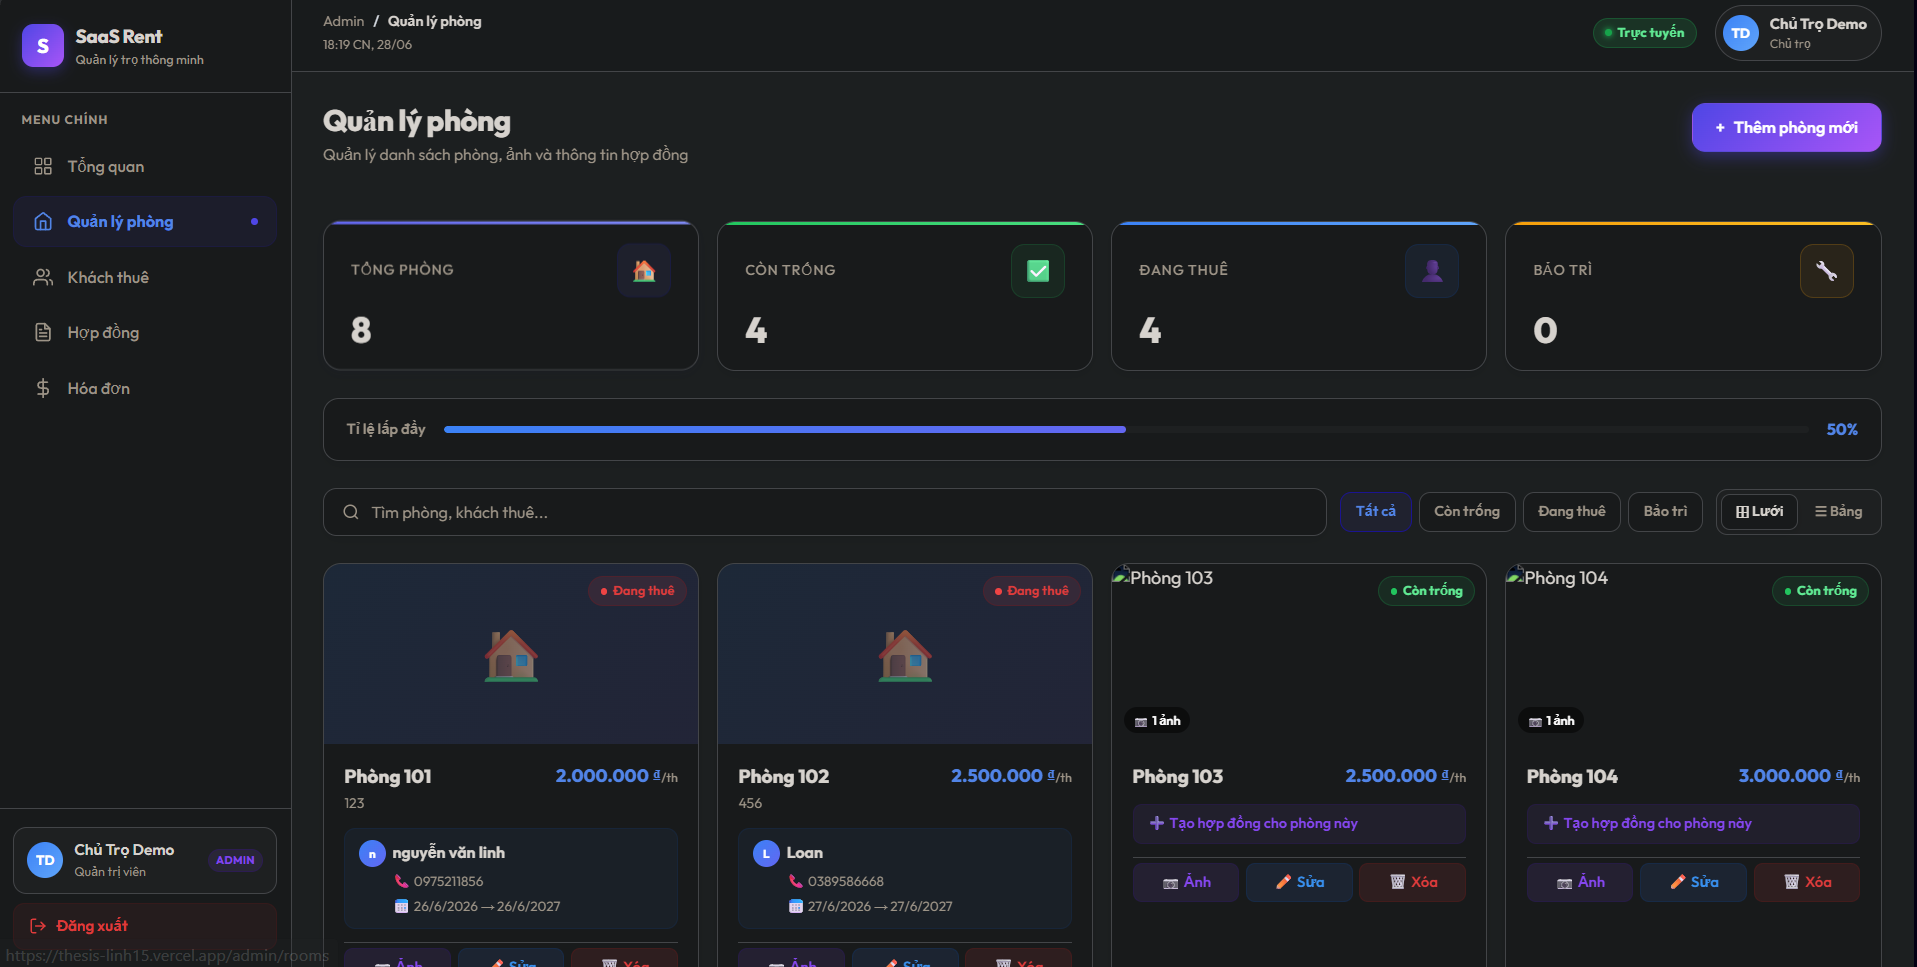
\includegraphics[width=0.95\textwidth]{landlord_room_management.png}
    \caption{Landlord Administration Dashboard — Room Management Overview}
    \label{fig:landlord_room_management}
\end{figure}

Below the statistics, the room list is displayed as a grid of cards. Each card shows the room number, the monthly rental price, and the current room status label. The status label uses colour-coded tags so that landlords can identify available and occupied rooms at a glance without reading individual details. A filter bar above the grid allows landlords to switch between viewing all rooms, only vacant rooms, only occupied rooms, or only rooms under maintenance. This filter makes it faster to locate specific rooms, especially when managing a large number of properties.

Each room card also contains quick-action buttons so that landlords can navigate directly to that room's detail, edit its information, or perform other operations without returning to the main menu. A prominent \textit{Thêm phòng mới} (Add New Room) button is placed in the top-right corner of the page, allowing landlords to register a new room at any time. When a landlord creates or updates a room, the system validates all required fields on the backend before saving. Room images are uploaded to the \textbf{Cloudinary} cloud service and the secure image URLs are stored in the \textbf{PostgreSQL} database, which ensures that room photos load quickly for public visitors without consuming local server storage.

\section{Public Room Listing and RentBot AI Chatbot}

The public-facing listing page is the entry point for people searching for a room to rent. This page is accessible without any login and is designed to attract potential tenants by presenting available rooms clearly. As shown in Figure \ref{fig:public_listing_rentbot}, the listing page displays a grid of room cards, each showing the room number, the monthly rental price in Vietnamese dong, and a \textit{CÒN TRỐNG} (Available) tag that confirms the room is currently unoccupied. In the example, three rooms are visible: Phòng 103 at 2{,}500{,}000 VND, Phòng 104 at 3{,}000{,}000 VND, and Phòng 203 at 3{,}500{,}000 VND. Each card has a \textit{Đăng ký phòng ngay} (Register for this room now) button that leads visitors to the room application form.

\begin{figure}[H]
    \centering
    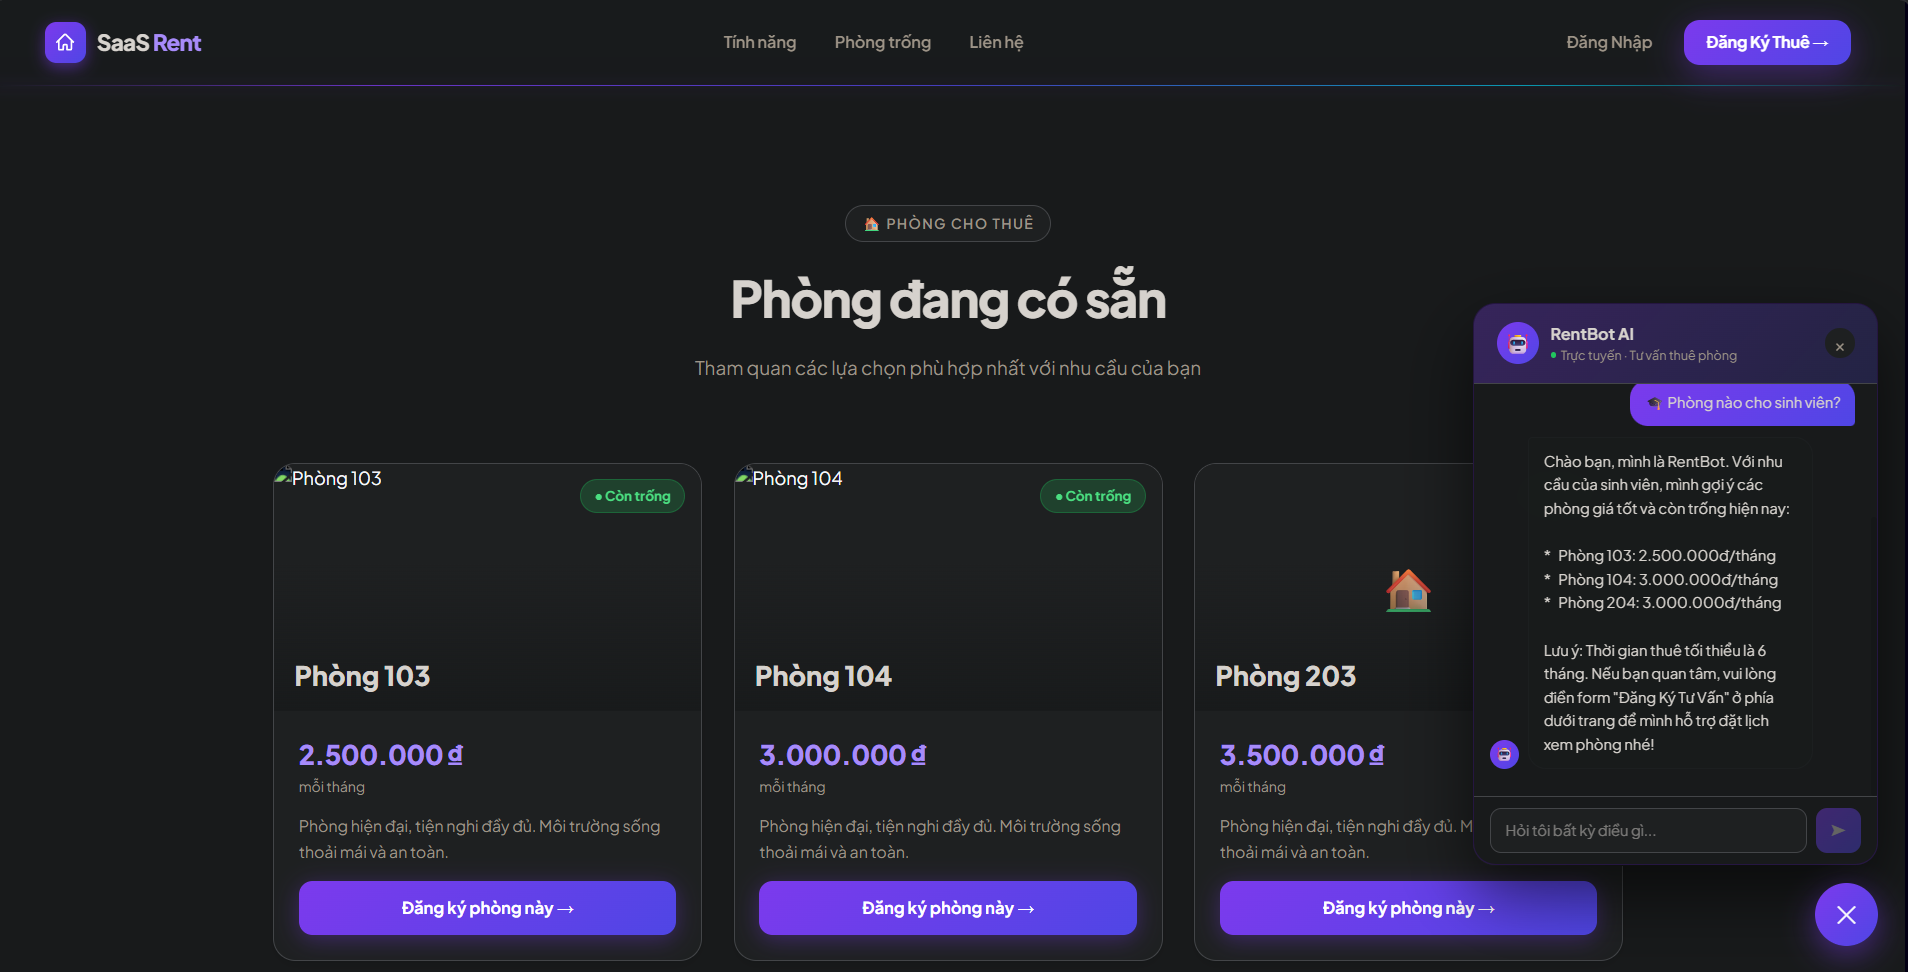
\includegraphics[width=0.95\textwidth]{public_listing_rentbot.png}
    \caption{Public Room Listing Page with RentBot AI Chatbot}
    \label{fig:public_listing_rentbot}
\end{figure}

The most notable feature on this page is the \textbf{RentBot} chatbot widget, visible as a floating panel on the right side of the screen. RentBot is a context-aware \textbf{AI} assistant powered by the \textbf{Google Gemini} model. When a visitor opens the chatbot, the backend first queries the \textbf{PostgreSQL} database to fetch the current list of available rooms, including their room numbers, prices, floors, and descriptions. This real-time room data is then inserted into the system prompt as context before the visitor's question is sent to the \textbf{Gemini} model. As demonstrated in the screenshot, RentBot successfully responds to the visitor by listing the available rooms with their correct prices and advising the visitor to use the registration button to apply. Because the assistant reads from live database records, it can never provide incorrect or outdated room information. This approach directly addresses the common problem of prospective tenants receiving inconsistent room availability information.

\section{Tenant Portal and Personal AI Assistant}

Once a tenant has been registered by a landlord and logs in to the system, they are directed to the tenant portal. The tenant portal is a private space where each tenant can monitor all aspects of their rental relationship. As shown in Figure \ref{fig:tenant_portal_dashboard}, the portal greets the tenant by name and displays the current date at the top of the page, providing a personalized and welcoming experience.

\begin{figure}[H]
    \centering
    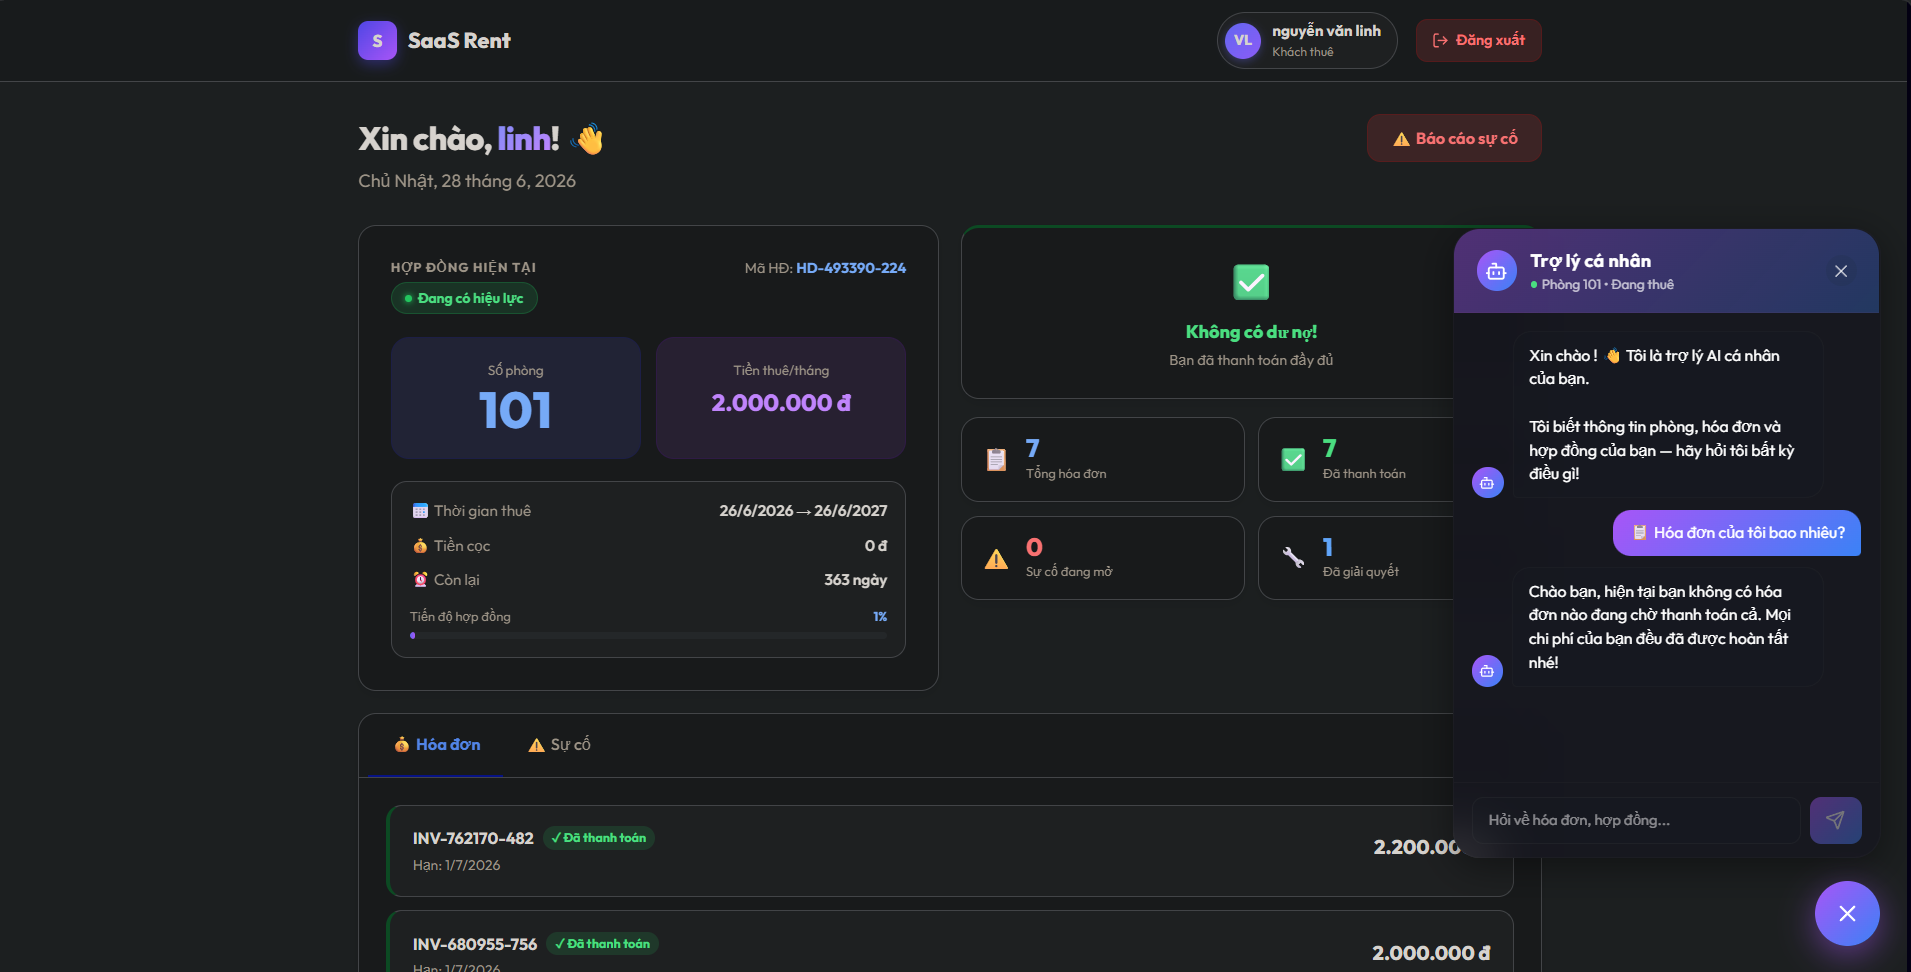
\includegraphics[width=0.95\textwidth]{tenant_portal_dashboard.png}
    \caption{Tenant Portal Dashboard with Contract Summary and Personal AI Assistant}
    \label{fig:tenant_portal_dashboard}
\end{figure}

The left section of the portal displays the tenant's current active contract in a summary card labelled \textit{Hợp đồng hiện tại} (Current Contract). This card shows the contract status, the room number the tenant is renting (Room 101 in this example), the rental start and end dates, and the number of days remaining on the contract. In the example shown, the tenant has a contract running from 24 June 2025 to 24 June 2027, with 363 days remaining. The tenant can also see the deposit amount and the monthly rental fee at a glance. Below the contract summary, the portal displays a list of recent invoices. Each invoice entry shows the invoice reference number, its payment status (such as \textit{Chờ thanh toán} meaning Pending, or \textit{Đã thanh toán} meaning Paid), and the invoice amount. This gives tenants a complete, up-to-date view of their billing history without needing to contact the landlord.

On the right side of the portal, a summary panel shows the tenant's activity counts, including the number of invoices already paid and the number of reported incidents that have been resolved. Two action buttons are placed prominently in the top-right corner: a \textit{Báo cáo sự cố} (Report Incident) button for submitting maintenance requests, and the \textit{Trợ lý cá nhân} (Personal Assistant) button that opens the AI chatbot.

The personal AI assistant is the most advanced feature of the tenant portal. When the tenant clicks the assistant button, the backend service queries the database to retrieve the tenant's active contract details, their full invoice history, any open incidents, and any recorded violations. All of this personal data is formatted as a structured system context and sent to the \textbf{Google Gemini} model together with the tenant's question. As demonstrated in the screenshot, the assistant can answer specific questions about the tenant's rental situation, such as informing the tenant about upcoming payment deadlines, explaining the amount still owed, or confirming whether an incident has been resolved. This level of personalization allows tenants to get precise, factual answers without calling or messaging the landlord directly.

\section{Invoice Payment with VietQR Integration}

The invoice payment workflow is one of the most practically important features of the system for both landlords and tenants. When a tenant views a pending invoice and clicks the payment button, the system opens a dedicated payment modal, as shown in Figure \ref{fig:invoice_payment_modal}. This modal presents all the information a tenant needs to complete a bank transfer, without requiring them to search for the landlord's bank details manually.

\begin{figure}[H]
    \centering
    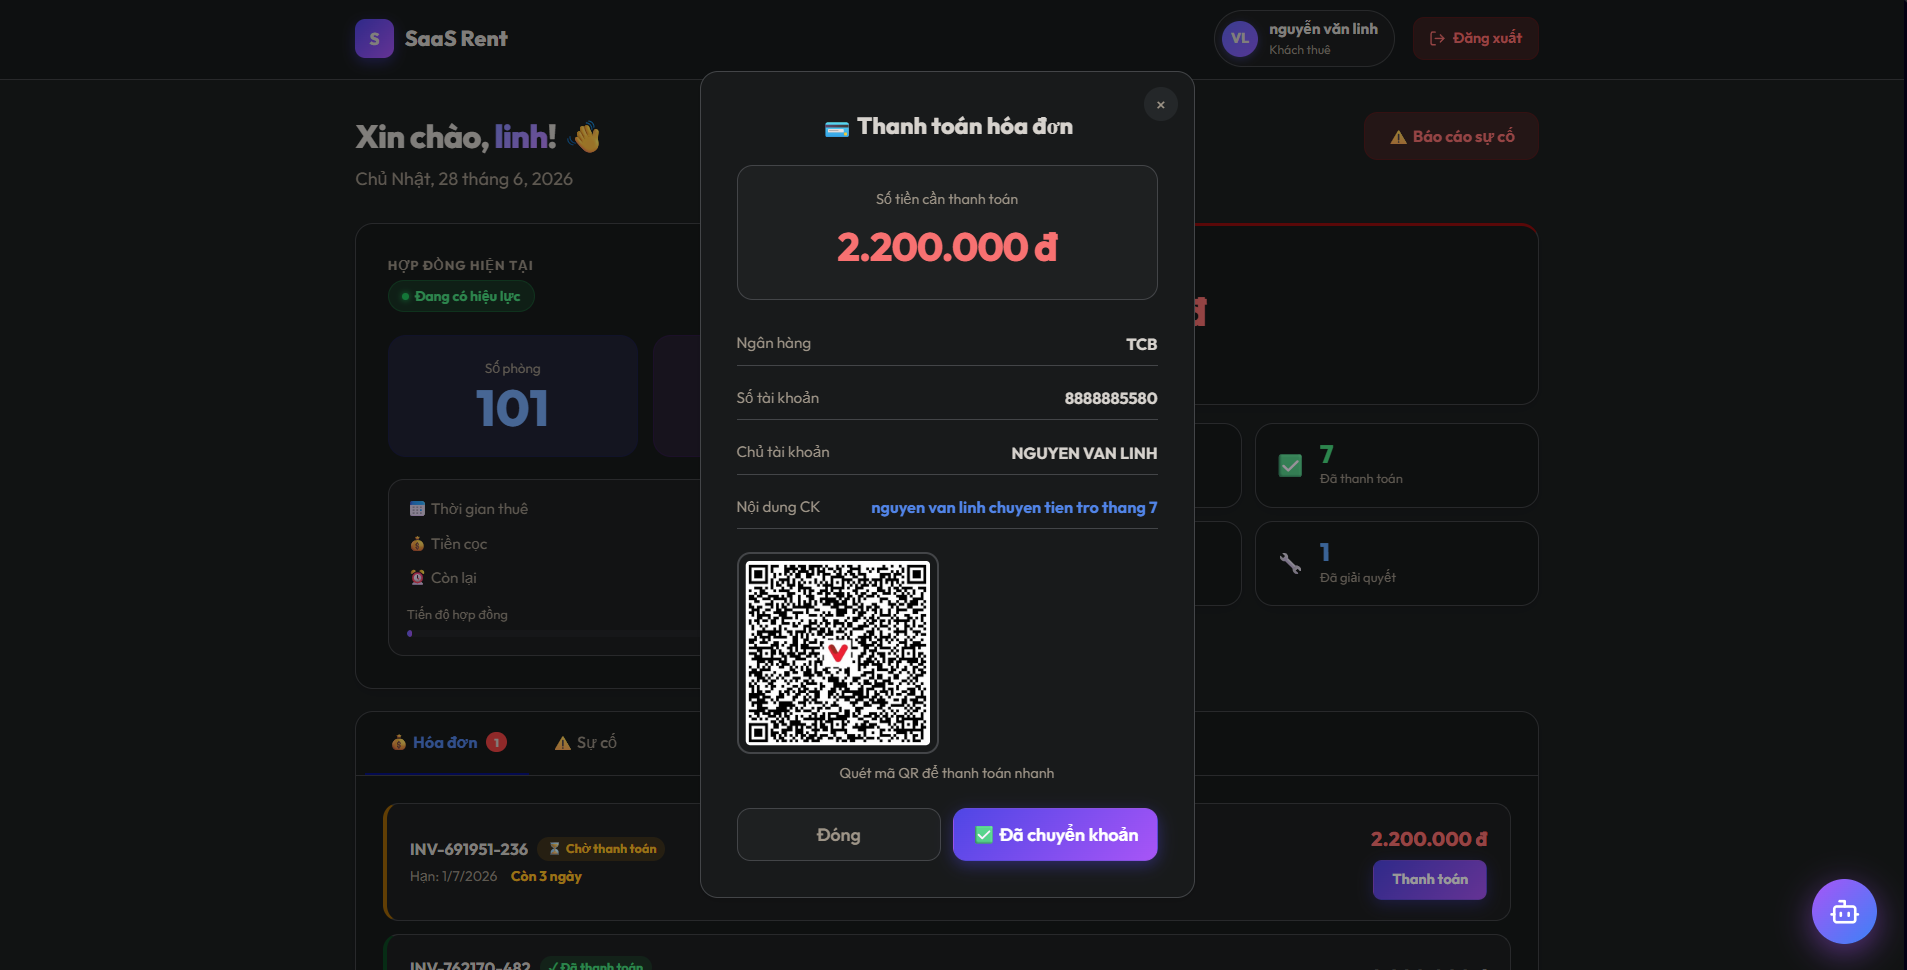
\includegraphics[width=0.75\textwidth]{invoice_payment_modal.png}
    \caption{Invoice Payment Modal with VietQR Code and Bank Transfer Details}
    \label{fig:invoice_payment_modal}
\end{figure}

At the top of the modal, the exact amount to be paid is displayed in large text, making it immediately clear to the tenant. In the example, the tenant must pay 2{,}200{,}000 VND for the current month. Below the amount, the modal shows the complete bank transfer details: the bank name (Techcombank, abbreviated as TCB), the bank account number (8888885580), and the account holder name (NGUYEN VAN LINH). These details are retrieved from the landlord's profile stored in the database.

The most significant element of the payment modal is the automatically generated \textbf{VietQR} code displayed in the centre. This QR code is produced dynamically by the \textbf{VietQR} image API using the landlord's bank account information and the specific invoice amount. The transfer memo (Nội dung CK) is also pre-filled automatically to include the tenant's name and the invoice month, so the landlord can easily identify which payment belongs to which tenant and which month. In the example, the memo reads \textit{nguyễn văn linh chuyển tiền trợ tháng 7} (Nguyen Van Linh transfers rent for month 7). The tenant only needs to open their mobile banking application and scan this QR code to complete the full bank transfer in seconds.

After transferring the money, the tenant clicks the \textit{Đã chuyển khoản} (Already Transferred) button at the bottom of the modal. This action sends a request to the backend, which immediately updates the invoice status to \textbf{Paid} and records the payment timestamp in the database. Simultaneously, the backend broadcasts a real-time \textbf{Socket.IO} WebSocket notification to the landlord's active dashboard session, informing them that a payment has been submitted. The landlord can then open their bank application separately to verify that the transfer was received, and manually confirm or adjust the invoice status if necessary. Table \ref{tab:implemented_features} provides a full summary of all core features implemented in the prototype.

\begin{table}[H]
    \centering
    \renewcommand{\arraystretch}{1.2}
    \begin{tabular}{|l|l|p{7cm}|}
        \hline
        \textbf{Feature} & \textbf{Status} & \textbf{Result} \\
        \hline
        Room CRUD and image upload & Implemented & Landlords manage room records with photos stored on Cloudinary. \\
        \hline
        Public room listing & Implemented & Vacant rooms are shown on the public page for prospective tenants. \\
        \hline
        RentBot public chatbot & Implemented & AI assistant answers room availability questions using live database context. \\
        \hline
        Contract creation & Implemented & Contracts are created with atomic room status synchronization. \\
        \hline
        Monthly invoice generation & Implemented & Scheduled cron task creates unpaid invoices for all active contracts. \\
        \hline
        VietQR payment modal & Implemented & Payment modal displays bank details and a dynamically generated QR code. \\
        \hline
        Invoice payment tracking & Implemented & Tenants mark invoices paid; landlords receive real-time notifications. \\
        \hline
        Tenant portal dashboard & Implemented & Tenants view their contract summary, invoice history, and incident status. \\
        \hline
        Personal AI assistant & Implemented & AI assistant answers tenant questions using personal contract and invoice data. \\
        \hline
        Incident reporting & Implemented & Tenants submit repair requests; landlords manage and resolve them. \\
        \hline
        Real-time notifications & Implemented & Socket.IO broadcasts events to the landlord dashboard without page reload. \\
        \hline
    \end{tabular}
    \caption{Summary of Implemented System Features}
    \label{tab:implemented_features}
\end{table}

\section{Difficulties and Limitations}

Although the prototype successfully implements all planned core features, several limitations must be acknowledged before the system can be considered ready for production deployment.

\textbf{Lack of automated testing.} The current codebase does not include comprehensive unit tests or integration tests. Automated testing is especially important for verifying complex business workflows such as the contract creation transaction, the monthly invoice generation cron job, and the multi-tenant authorization filters. Without these tests, adding new features in the future carries a higher risk of accidentally breaking existing behaviour.

\textbf{Manual payment verification.} The invoice payment workflow requires the landlord to verify bank transfers manually by checking their bank application separately. Because the system is not connected to a live banking webhook or an open banking API, it cannot automatically detect and confirm incoming payments. The tenant must click the \textit{Already Transferred} button to update the invoice status, and the landlord must independently confirm the transfer. This introduces a risk of human error and delays in payment confirmation.

\textbf{Dependency on external AI service.} All three \textbf{AI} assistant features — the notice generator, the public RentBot, and the personal tenant assistant — depend entirely on the external \textbf{Google Gemini} API. If the Google service is temporarily unavailable, rate-limited, or slow, the chatbot features will fail or respond with significant delays, directly reducing the reliability of the system for users who depend on it.

\textbf{Multi-tenant security relies on application-level filtering.} Data privacy between landlords is enforced by filtering every database query using the landlord identification code extracted from the \textbf{JWT} token. While this approach works correctly in the current implementation, a production-grade SaaS platform should also implement database-level row security policies and audit logging to guard against potential code-level mistakes that could expose one landlord's data to another.

\textbf{No mobile application.} The platform is built as a responsive web application accessible through a browser. However, tenants and landlords in Vietnam predominantly use smartphones for day-to-day activities, and a dedicated mobile application would provide a significantly smoother experience, especially for scanning QR codes and receiving push notifications.

\section{Discussion}

The results of this project demonstrate that a fully integrated web-based boarding house management platform can be built using modern open-source technologies and cloud services within the scope of a single undergraduate thesis project. By combining a modular \textbf{NestJS} backend, a server-rendered \textbf{Next.js} frontend, a \textbf{PostgreSQL} relational database, and the \textbf{Google Gemini} AI model, the system delivers a coherent set of features that directly address the real-world problems described in Chapter 1.

The most significant technical achievement is the integration of multiple system components into seamless end-to-end workflows. For example, the room status in the database changes automatically when a contract is created, expires, or is terminated. Monthly invoices are generated without any manual intervention from the landlord through the scheduled cron job. When a tenant submits payment confirmation, the landlord's dashboard is updated instantly through the \textbf{Socket.IO} WebSocket connection without requiring a page refresh. These automated workflows eliminate manual data entry, reduce the chance of human error, and save considerable time for landlords managing multiple rooms simultaneously.

The \textbf{AI} integration proves to be one of the most practical additions to the system. The public \textbf{RentBot} reduces the number of repetitive inquiries that landlords must answer by allowing visitors to ask questions about available rooms directly on the listing page. The personal tenant assistant gives tenants a self-service channel for checking their contract terms, outstanding bills, and incident status at any time, without needing to contact the landlord. Both assistants use live data from the database rather than static scripts, which ensures that the answers are always accurate and up-to-date.

The multi-tenant architecture design ensures that the platform can serve multiple landlords from a single deployed instance without any risk of data leakage between users. Each landlord's rooms, tenants, contracts, and invoices are fully isolated through consistent use of the landlord identification code as a query filter on every database operation. This design is scalable and aligns with the SaaS business model described in the objectives of this thesis.

In conclusion, the implemented prototype successfully validates the design decisions made in Chapter 4 and fulfills the functional requirements defined in Chapter 3. The limitations identified — particularly the absence of automated tests, manual payment verification, and external AI dependency — are well-understood trade-offs that are appropriate for a prototype at this stage. Addressing these limitations through automated testing, open banking API integration, and AI fallback strategies would be the natural next steps for transforming this prototype into a production-ready product.

\chapter{CONCLUSION AND FUTURE WORK}

This chapter summarizes the final results of this bachelor thesis and outlines the main future directions to improve the system.

\section{Conclusion}
The \textit{\textbf{Smart Boarding House Management System}} successfully provides a practical foundation for digitizing rental property operations. The project solves common problems in boarding house management by centralizing room details, tenant registration, contracts, invoices, payment tracking, incidents, violations, rent requests, notifications, and AI support in a single \textbf{SaaS} platform.

From a software engineering perspective, the project demonstrates that combining modular design with clean architecture rules makes codebases highly maintainable. The backend built with \textbf{NestJS} and \textbf{Prisma ORM} ensures that database operations in \textbf{PostgreSQL} are secure and consistent. The use of custom guards like the \textbf{JwtAuthGuard} and \textbf{RolesGuard} protects private API endpoints. On the frontend, \textbf{Next.js} and \textbf{Zustand} provide a modular portal interface. The integration of supporting services like \textbf{Socket.IO} for notifications, \textbf{Cloudinary} for uploads, and \textbf{Google Gemini} for AI chat completes a modern development package. This prototype represents a secure, maintainable, and solid base for a commercial rental application.

\section{Future Work}
Although the prototype works successfully, several technical improvements can be added in future versions to make it ready for production.

\subsection{Production Payment Integration}
The current payment verification process is manual. To automate this, the system should integrate payment gateway APIs such as \textbf{PayOS}, \textbf{MoMo}, or \textbf{VNPay} and listen to secure database webhooks. When a tenant scans the \textbf{VietQR} code and transfers money, the payment provider will automatically send a secure HTTP post request to the backend. The backend will parse the webhook, verify the invoice ID, update the invoice status to paid, and send an instant notification to both the landlord and tenant, eliminating manual verification.

\subsection{Advanced Utility Billing}
The utility billing module can be improved by tracking consumption history. Future versions should save previous and current meter readings in the database, allowing the system to calculate the difference between readings and automatically compute the electricity or water cost. The system can also run consistency checks to warn the landlord if a room has abnormally high consumption compared to previous months.

\subsection{Stronger Multi-Tenant Security}
To prepare for large-scale SaaS deployment, database-level security must be hardened. Future work should implement **Row-Level Security (RLS)** in \textbf{PostgreSQL} to enforce isolation at the database layer. Additionally, the backend should include security auditing logs to record database queries, rate limiters using the NestJS throttler module to prevent automated attacks, and strict origin checks on WebSockets to secure real-time connections.

\subsection{Mobile Tenant Experience}
Tenants primarily use mobile phones to interact with the boarding house system. Developing a native mobile application using \textbf{React Native} or \textbf{Flutter}, or converting the frontend into a \textbf{Progressive Web App (PWA)}, will make it much easier for tenants to view bills and report incidents. This will also allow the system to send mobile push notifications directly to the tenant's lock screen when a new invoice is created.

\subsection{Analytics and Forecasting}
The landlord dashboard can be expanded with analytics to track business performance. The system can calculate metrics like monthly recurring revenue, overall occupancy rate, average repair resolution times, and outstanding debts. Furthermore, machine learning models or Gemini forecasting can analyze historical data to help landlords predict vacancy risks and manage cash flow.

\subsection{Document and Contract Management}
The document management features can be expanded to include paperless contract signing. The backend can generate PDF lease documents dynamically and integrate electronic signature services like \textbf{DocuSign} or local digital signature certificates. This will allow landlords and tenants to sign contracts digitally, making them legally binding and securely stored in the system.


\bibliographystyle{plainurl}
\bibliography{references}
\nocite{*}

\end{document}
